% =====================================================================
%  TA-IND-01 — Aplicaciones Distribuidas
%  Análisis crítico de Redis Cluster comparado con Hazelcast
%  Autor: Sánchez Vera Darwin Joel
%  Compilación (desde la carpeta informe/):
%    pdflatex main  ->  biber main  ->  pdflatex main  ->  pdflatex main
% =====================================================================
\documentclass[11pt,a4paper]{article}

% ---------- Idioma y codificación ----------
\usepackage[T1]{fontenc}
\usepackage[utf8]{inputenc}
\usepackage[english,spanish,es-tabla,es-nodecimaldot]{babel}
\usepackage{lmodern}
\usepackage{microtype}

% ---------- Página ----------
\usepackage[margin=2.5cm]{geometry}
\usepackage{setspace}
\onehalfspacing
\usepackage{parskip}

% ---------- Tablas, figuras y código ----------
\usepackage{graphicx}
\graphicspath{{../figuras/}{../capturas/sistema/}{../capturas/lecturas/}}
\usepackage{float}
\usepackage{booktabs}
\usepackage{tabularx}
\usepackage{array}
\usepackage{caption}
\usepackage[table]{xcolor}
\usepackage{listings}
\lstset{
  basicstyle=\ttfamily\small,
  breaklines=true,
  frame=single,
  backgroundcolor=\color{gray!8},
  columns=fullflexible,
  keepspaces=true
}

% ---------- Bibliografía (IEEE + biber) ----------
\usepackage[style=ieee, backend=biber, language=english]{biblatex}
\usepackage{xpatch}
% Evita "()" vacíos en las entradas @online sin fecha
\xpatchbibdriver{online}{\printtext[parens]{\usebibmacro{date}}}%
  {\iffieldundef{year}{}{\printtext[parens]{\usebibmacro{date}}}}{}{}
\addbibresource{referencias.bib}

% ---------- Enlaces ----------
\usepackage{hyperref}
\hypersetup{colorlinks=true, urlcolor=blue, linkcolor=black, citecolor=black}
\usepackage{csquotes}

% =====================================================================
\begin{document}

% ---------------------------- Carátula ----------------------------
\begin{titlepage}
  \centering
  {\Large\bfseries UNIVERSIDAD TÉCNICA ESTATAL DE QUEVEDO\par}
  \vspace{0.3cm}
  {\large Facultad de Ciencias de la Computación y Diseño Digital\par}
  {\large Carrera de Ingeniería de Software\par}
  \vspace{2cm}
  {\large\bfseries Aplicaciones Distribuidas\par}
  \vspace{0.3cm}
  {\large Actividad individual TA-IND-01\par}
  \vspace{1.5cm}
  {\LARGE\bfseries Análisis crítico de Redis Cluster como sistema distribuido\\[0.2cm]
   y comparación con Hazelcast\par}
  \vspace{2cm}
  \begin{tabular}{rl}
    \textbf{Estudiante:} & Sánchez Vera Darwin Joel \\
    \textbf{Correo:}     & dsanchezv@uteq.edu.ec \\
    \textbf{Docente:}    & GUERRERO ULLOA GLEISTON CICERON \\
    \textbf{Curso / paralelo:} & 7mo B \\
    \textbf{Repositorio:} & \url{https://github.com/DarwinDevCode/REPO-TA-IND-01} \\
  \end{tabular}
  \vfill
  {\large Quevedo, Ecuador\\ 15 de noviembre de 2026\par}
\end{titlepage}

% ---------------------------- Resumen ----------------------------
\begin{abstract}
PENDIENTE
\end{abstract}

\tableofcontents
\newpage

% =====================================================================
\section{Introducción}
% =====================================================================

Las aplicaciones actuales necesitan acceder a datos en pocos milisegundos y
seguir funcionando aunque falle alguno de sus servidores. Para lograrlo, los
datos se reparten y se replican entre varias máquinas, lo que convierte al
almacén de datos en un sistema distribuido con todos sus problemas: fallos
parciales, comunicación por red y la necesidad de decidir cuánta consistencia
se puede ofrecer sin perder disponibilidad ni rendimiento
\cite{vansteen2023distributed, ahmed2023consistency}.

Redis es un almacén clave--valor en memoria muy utilizado como caché, gestor
de sesiones y cola ligera. Su modo distribuido, \emph{Redis Cluster}, reparte
las claves entre varios nodos maestros mediante \emph{hash slots}, mantiene
réplicas de cada maestro y promueve una réplica de forma automática cuando un
maestro falla \cite{redis2026clusterspec, redis2026scaling}. Desde mayo de 2025
Redis vuelve a distribuirse con una licencia de código abierto (AGPLv3), lo que
facilita estudiarlo y desplegarlo libremente \cite{trollope2025agpl}. Su uso a
gran escala también ha mostrado sus riesgos: en marzo de 2023 un fallo en la
biblioteca cliente de Redis provocó que algunos usuarios de ChatGPT vieran
datos de otros usuarios \cite{openai2023outage}.

El objetivo de este informe es analizar Redis Cluster con los conceptos de la
Unidad~1 de la asignatura (transparencias de distribución, teoremas CAP y
PACELC, modelos de comunicación y tolerancia a fallos) y compararlo con
Hazelcast, una plataforma de datos en memoria que reparte sus datos en
particiones con copias de respaldo y que, además, ofrece un subsistema de
consistencia fuerte basado en Raft \cite{hazelcast2026partitioning,
hazelcast2026cpsubsystem}. El análisis se apoya en la documentación oficial,
en artículos científicos recientes y en un clúster real de seis nodos
desplegado con Docker, sobre el que se realizó un experimento de caída de un
nodo maestro.

El informe se organiza así: la Sección~\ref{sec:arquitectura} describe la
arquitectura del clúster desplegado; la Sección~\ref{sec:unidad1} analiza
Redis Cluster con los conceptos de la Unidad~1; la
Sección~\ref{sec:experimentacion} presenta la experimentación propia; la
Sección~\ref{sec:comparacion} compara Redis Cluster con Hazelcast; la
Sección~\ref{sec:postura} expone una postura crítica, y la
Sección~\ref{sec:conclusiones} resume las conclusiones.

% =====================================================================
\section{Arquitectura de Redis Cluster}
\label{sec:arquitectura}
% =====================================================================

\subsection{Componentes principales}

\textbf{Hash slots.} Redis Cluster no reparte las claves con un hashing
consistente clásico, sino con un espacio fijo de 16\,384 \emph{hash slots}.
Cada clave pertenece al slot $\mathrm{CRC16}(\mathit{clave}) \bmod 16384$, y
cada nodo maestro es responsable de un subconjunto de slots
\cite{redis2026clusterspec}. Si una clave contiene un \emph{hash tag} entre
llaves (por ejemplo, \texttt{\{usuario:25\}:perfil}), solo se usa la parte
entre llaves para calcular el slot, lo que permite forzar que varias claves
queden en el mismo nodo.

\textbf{Maestros y réplicas.} Cada maestro atiende las lecturas y escrituras
de sus slots y tiene una o más réplicas que reciben una copia de sus datos de
forma \emph{asíncrona} \cite{redis2026replication}. Las réplicas no atienden
escrituras; su función principal es sustituir al maestro si este falla.

\textbf{Bus del clúster.} Además del puerto de clientes (6379), cada nodo
abre un segundo puerto (el de clientes más 10\,000, es decir, 16379) para el
\emph{cluster bus}: una malla en la que todos los nodos están conectados con
todos y se envían mensajes binarios de \emph{ping/pong}. Por este bus se
propaga, mediante \emph{gossip}, la configuración del clúster (qué nodo es
dueño de qué slots) y se detectan los fallos \cite{redis2026clusterspec}.

\textbf{Clientes y redirección.} No existe un proxy ni un nodo coordinador.
El cliente puede enviar una petición a cualquier nodo; si ese nodo no es el
dueño del slot, responde con un error \texttt{MOVED} que indica el slot y la
dirección del nodo correcto, y el cliente repite la petición allí. Durante una
migración de slots se usa la redirección temporal \texttt{ASK}
\cite{redis2026clusterspec}.

\subsection{Clúster desplegado}

Para este trabajo se desplegó un clúster de seis contenedores Docker
(\texttt{redis:8}) en la red \texttt{redisnet} (172.30.0.0/16), creado con
\texttt{redis-cli --cluster create} y la opción \texttt{--cluster-replicas 1}.
La Tabla~\ref{tab:nodos} muestra la distribución resultante y la
Figura~\ref{fig:arquitectura} la arquitectura completa.

\begin{table}[H]
  \centering
  \caption{Distribución de slots y réplicas en el clúster desplegado.}
  \label{tab:nodos}
  \begin{tabular}{llll}
    \toprule
    \textbf{Maestro} & \textbf{IP} & \textbf{Slots} & \textbf{Réplica} \\
    \midrule
    redis-1 (A) & 172.30.0.11 & 0 -- 5460      & redis-5 (172.30.0.15) \\
    redis-2 (B) & 172.30.0.12 & 5461 -- 10922  & redis-6 (172.30.0.16) \\
    redis-3 (C) & 172.30.0.13 & 10923 -- 16383 & redis-4 (172.30.0.14) \\
    \bottomrule
  \end{tabular}
\end{table}

\begin{figure}[H]
  \centering
  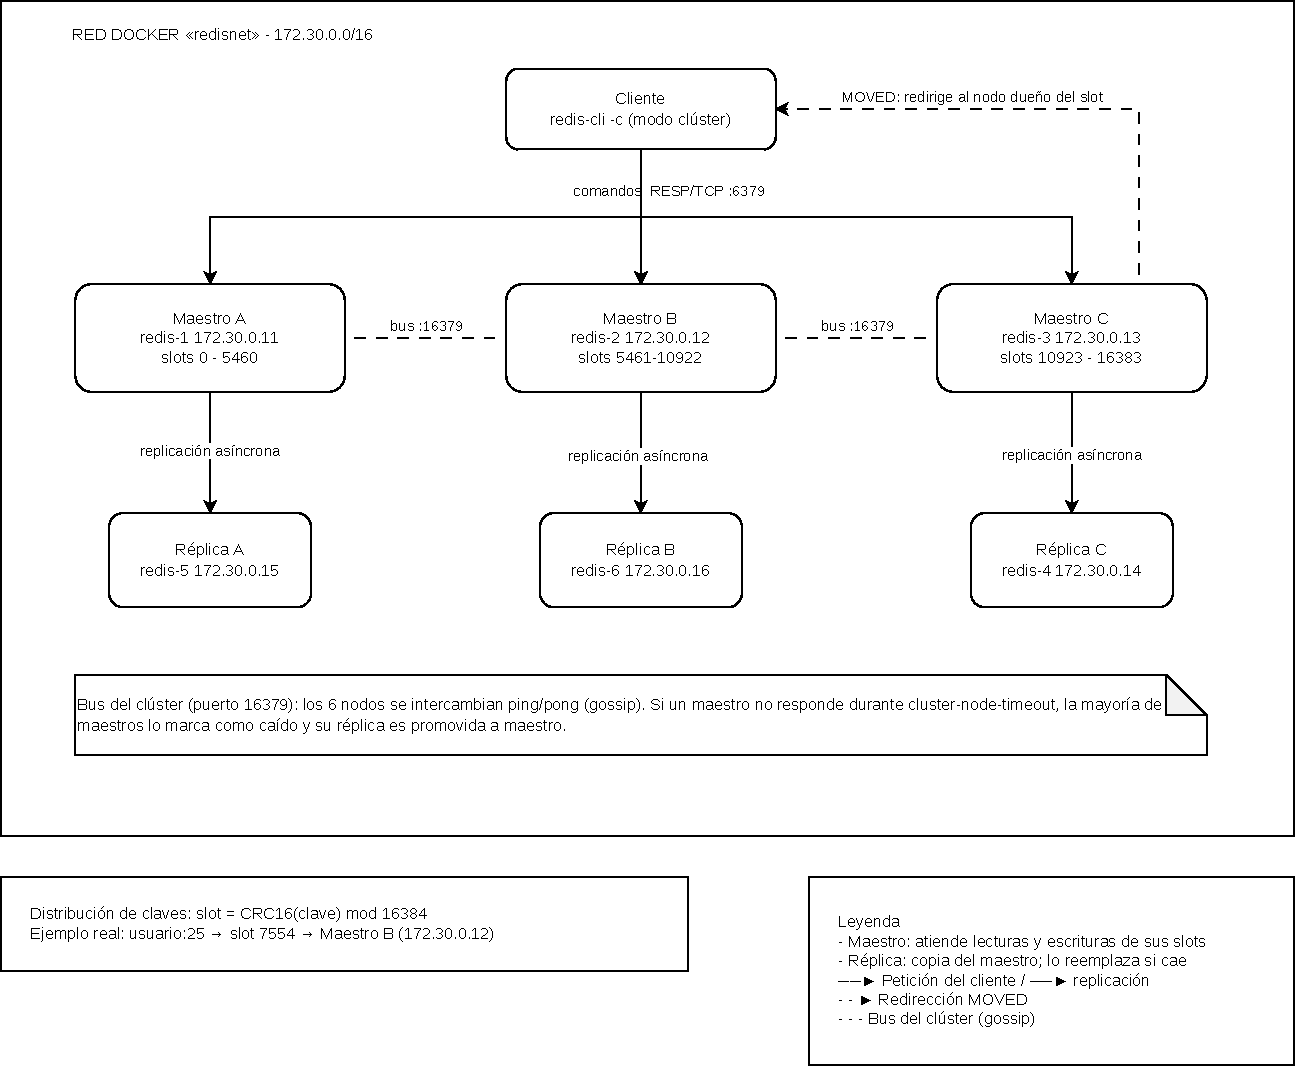
\includegraphics[width=\linewidth]{diagrama_arquitectura.pdf}
  \caption{Arquitectura del clúster Redis desplegado: red \texttt{redisnet},
  tres maestros con sus rangos de slots, tres réplicas con replicación
  asíncrona, bus del clúster (puerto 16379) y redirección \texttt{MOVED}.
  Elaboración propia en draw.io.}
  \label{fig:arquitectura}
\end{figure}

Por ejemplo, la clave \texttt{usuario:25} cae en el slot 7554, que pertenece
al maestro B (172.30.0.12), y la clave \texttt{materia:aplicaciones} cae en el
slot 13574, que pertenece al maestro C (172.30.0.13). Al conectarse a
\texttt{redis-1}, el cliente recibió en ambos casos una redirección hacia el
nodo dueño del slot (Figura~\ref{fig:redireccion}, Sección~\ref{sec:experimentacion}).

\subsection{Evolución del diseño}

El diseño de la arquitectura partió de un esquema dibujado a mano (Anexo~A,
Figura~\ref{fig:anexoA}) y se refinó en el diagrama final de la
Figura~\ref{fig:arquitectura}.

El boceto se dibujó el 13 de noviembre de 2026, antes de desplegar el clúster,
a partir de la lectura de la especificación oficial. Recoge la idea general
de la arquitectura: un cliente (la aplicación), tres maestros con sus rangos
de slots (0--5460, 5461--10922 y 10923--16383), una réplica por maestro que
recibe una ``copia'' de sus datos y una comunicación entre nodos representada
con flechas punteadas. Sin embargo, al contrastarlo con el clúster real se
identificaron varias carencias:

\begin{itemize}
  \item \textbf{El cliente parecía enviar cada petición a los tres
  maestros.} La flecha ``petición'' se ramificaba hacia todos ellos. En
  realidad el cliente envía cada comando a un solo nodo y, si ese nodo no es
  el dueño del slot, recibe una redirección \texttt{MOVED}. El boceto no
  mostraba esta redirección, que es la base de la transparencia de ubicación.
  \item \textbf{La copia no indicaba cómo se replica.} La flecha ``copia'' no
  distinguía entre replicación síncrona y asíncrona, que es justamente lo que
  determina si Redis puede perder escrituras (Sección~\ref{sec:unidad1}).
  \item \textbf{La comunicación entre nodos estaba incompleta.} Las líneas
  punteadas solo unían A con B y B con C, como si fuera una cadena, y no
  indicaban el puerto ni el tipo de mensaje. En realidad el bus del clúster
  conecta a los seis nodos entre sí por el puerto 16379.
  \item \textbf{Faltaban los datos reales.} No aparecían los contenedores, las
  direcciones IP ni la red en la que se ejecutan los nodos.
\end{itemize}

El diagrama final (Figura~\ref{fig:arquitectura}) corrige estos puntos con la
información obtenida al desplegar el clúster. Ubica todos los nodos dentro de
la red Docker \texttt{redisnet} e identifica cada nodo por su contenedor e IP.
Incorpora la asignación real de réplicas que hizo \texttt{redis-cli}, que no
siguió el orden de los contenedores: el maestro A quedó con
\texttt{redis-5}, el B con \texttt{redis-6} y el C con \texttt{redis-4}.
También distingue el tráfico de clientes (RESP/TCP, puerto 6379), el bus del
clúster (puerto 16379), la replicación asíncrona y la redirección
\texttt{MOVED}. Por último, añade una nota sobre la detección de fallos, la
fórmula de cálculo del slot con un ejemplo real del experimento y una leyenda
más completa. Por legibilidad, el diagrama solo dibuja el bus entre maestros
vecinos; la nota aclara que los seis nodos intercambian mensajes entre sí.

% =====================================================================
\section{Análisis de Redis Cluster según la Unidad 1}
\label{sec:unidad1}
% =====================================================================

\subsection{Transparencias de distribución}

Un sistema distribuido es transparente cuando oculta a usuarios y
aplicaciones que sus procesos y recursos están repartidos entre varias
máquinas \cite{vansteen2023distributed}. Redis Cluster ofrece varias de estas
transparencias, pero casi todas de forma \emph{parcial}, como resume la
Tabla~\ref{tab:transparencias}.

\begin{table}[H]
  \centering
  \caption{Transparencias de distribución en Redis Cluster.}
  \label{tab:transparencias}
  \small
  \begin{tabularx}{\linewidth}{>{\bfseries}l c X}
    \toprule
    \textbf{Transparencia} & \textbf{Nivel} & \textbf{Justificación} \\
    \midrule
    Acceso & Parcial &
      Se usan los mismos comandos que en un Redis independiente, pero las
      operaciones con varias claves (\texttt{MSET}, \texttt{MULTI/EXEC},
      scripts Lua) solo funcionan si todas las claves están en el mismo slot;
      si no, el servidor responde con el error \texttt{CROSSSLOT}. \\
    Ubicación & Parcial &
      El cliente no necesita saber en qué nodo está una clave, pero debe ser
      un cliente ``consciente del clúster'' que interprete \texttt{MOVED} y
      \texttt{ASK}. Con \texttt{redis-cli} sin la opción \texttt{-c} la
      redirección llega al usuario como un error. \\
    Migración y reubicación & Parcial &
      Los slots pueden moverse entre nodos en caliente (\emph{resharding});
      durante la migración el cliente recibe \texttt{ASK} y debe reintentar
      en el nodo destino \cite{redis2026scaling}. \\
    Replicación & Alta &
      El cliente lee y escribe en el maestro sin ver las réplicas. Solo si
      quiere leer de una réplica debe pedirlo con \texttt{READONLY},
      aceptando datos posiblemente desactualizados \cite{redis2026replication}. \\
    Fallos & Parcial &
      Tras el \emph{failover} el cliente sigue trabajando sin cambios, pero
      durante la detección del fallo una parte de las claves no está
      disponible (en el experimento E1, unos 7.8\,s). \\
    Concurrencia & Alta &
      Cada nodo ejecuta los comandos uno a uno, por lo que cada comando es
      atómico y los clientes concurrentes no ven estados intermedios. \\
    \bottomrule
  \end{tabularx}
\end{table}

La conclusión es que Redis Cluster no intenta ocultar por completo la
distribución: traslada parte del trabajo al cliente (conocer el mapa de
slots, agrupar claves con \emph{hash tags}) a cambio de evitar un proxy o
coordinador central que añadiría latencia y un punto único de fallo.

\subsection{Teoremas CAP y PACELC}

El teorema CAP establece que, cuando se produce una partición de red (P), un
sistema replicado debe elegir entre responder con datos posiblemente
desactualizados, sacrificando la consistencia (C), o dejar de responder,
sacrificando la disponibilidad (A) \cite{ahmed2023consistency}. PACELC añade
que, incluso sin particiones (E, \emph{else}), existe un compromiso entre
latencia (L) y consistencia (C), porque mantener las réplicas sincronizadas
exige esperar su confirmación \cite{ahmed2023consistency}.

\textbf{Comportamiento ante particiones (PA).} Redis Cluster no garantiza
consistencia fuerte. La especificación oficial reconoce que el clúster puede
perder escrituras que ya confirmó al cliente, por dos motivos: la replicación
asíncrona y las particiones de red en las que un maestro aislado sigue
aceptando escrituras durante un tiempo \cite{redis2026clusterspec}. Un maestro
que queda en la minoría de una partición deja de aceptar escrituras solo
después de \texttt{cluster-node-timeout}; mientras tanto, la mayoría puede
promover a su réplica, y las escrituras recibidas por el maestro aislado se
pierden al reincorporarse. Es decir, durante una partición el sistema prefiere
seguir respondiendo antes que coordinarse, y por eso se clasifica como PA.

Es cierto que, por defecto, Redis Cluster deja de atender consultas en todo el
clúster si algún rango de slots queda sin maestro
(\texttt{cluster-require-full-coverage yes}), como se observó en el
experimento E1. Pero esa pérdida temporal de disponibilidad no compra
consistencia fuerte: solo evita responder con una vista incompleta de los
datos.

\textbf{Comportamiento sin particiones (EL).} En funcionamiento normal, el
maestro responde \texttt{OK} al cliente antes de enviar el cambio a sus
réplicas \cite{redis2026replication}. Se elige así la latencia sobre la
consistencia. El comando \texttt{WAIT} permite esperar a que un número de
réplicas confirme la escritura, pero no convierte a Redis en un sistema
fuertemente consistente: una réplica que no recibió la escritura todavía puede
ser promovida \cite{redis2026clusterspec}. Además, su coste es alto: en el
estudio de Ferreira et~al., configurar Redis para esperar a todas las réplicas
con \texttt{WAIT} redujo drásticamente el rendimiento de escritura,
especialmente cuando los nodos estaban en regiones distintas
\cite{ferreira2024impacts, ferreira2025benchmarking}.

Por estas razones, en este informe Redis Cluster se clasifica como
\textbf{PA/EL}. Esta clasificación difiere de la revisión de Ahmed et~al.,
que incluye a Redis entre los sistemas CP del teorema CAP
\cite[p.~172]{ahmed2023consistency}; esa diferencia se discute en la
Sección~\ref{sec:postura}.

\subsection{Modelos de comunicación}

En Redis Cluster conviven varios modelos de comunicación, cada uno con un
propósito distinto (Tabla~\ref{tab:comunicacion}).

\begin{table}[H]
  \centering
  \caption{Modelos de comunicación presentes en Redis Cluster.}
  \label{tab:comunicacion}
  \small
  \begin{tabularx}{\linewidth}{l l X}
    \toprule
    \textbf{Interacción} & \textbf{Modelo} & \textbf{Descripción} \\
    \midrule
    Cliente -- nodo & Petición--respuesta síncrona &
      El cliente envía comandos con el protocolo RESP sobre TCP (puerto 6379)
      y espera la respuesta. Las redirecciones \texttt{MOVED}/\texttt{ASK}
      forman parte de este intercambio. \\
    Nodo -- nodo & Mensajes asíncronos (\emph{gossip}) &
      Mensajes binarios \emph{ping/pong} por el bus del clúster (puerto
      16379). Cada mensaje lleva información sobre otros nodos, de modo que
      la configuración y los fallos se propagan sin un coordinador central
      \cite{redis2026clusterspec}. \\
    Maestro -- réplica & Flujo asíncrono de comandos &
      El maestro envía a la réplica el flujo de comandos de escritura sin
      esperar confirmación; si la conexión se corta, la réplica intenta una
      resincronización parcial o completa \cite{redis2026replication}. \\
    Publicador -- suscriptores & Publicación/suscripción &
      Comunicación no persistente: el mensaje solo llega a los suscriptores
      conectados en ese momento. En el clúster, \texttt{PUBLISH} se difunde
      por el bus a todos los nodos \cite{redis2026clusterspec}. \\
    \bottomrule
  \end{tabularx}
\end{table}

El diseño evita la comunicación síncrona entre servidores en el camino de
cada petición: el cliente habla con un único nodo, y la coordinación entre
nodos ocurre en segundo plano por el bus. Esto explica la baja latencia de
Redis Cluster, pero también por qué la información sobre fallos tarda unos
segundos en propagarse.

\subsection{Tolerancia a fallos}

\textbf{Detección de fallos.} Cada nodo envía \emph{pings} periódicos a los
demás por el bus del clúster. Si un nodo no responde durante más de
\texttt{cluster-node-timeout}, quien lo detecta lo marca como \texttt{PFAIL}
(posible fallo). Esa sospecha se difunde por \emph{gossip}, y cuando la
mayoría de los maestros la reporta, el estado pasa a \texttt{FAIL} y se
propaga a todo el clúster \cite{redis2026clusterspec}.

\textbf{Recuperación (failover).} Cuando un maestro está en \texttt{FAIL},
sus réplicas solicitan el voto de los demás maestros. La réplica que obtiene
la mayoría incrementa su \emph{configEpoch}, se declara nuevo maestro de los
slots y anuncia la nueva configuración; ante configuraciones en conflicto,
gana la de época más alta. Si el antiguo maestro vuelve, se reincorpora como
réplica del nuevo \cite{redis2026clusterspec}. En el experimento E1 este
proceso tardó 7.8\,s con un \texttt{cluster-node-timeout} de 5\,s, y la época
de configuración del nuevo maestro pasó de 2 a 7
(Sección~\ref{sec:experimentacion}).

\textbf{Límites de la tolerancia a fallos.} El mecanismo tolera la caída de
un maestro mientras tenga una réplica disponible y la mayoría de maestros siga
activa. No protege frente a la pérdida de escrituras recientes, ya que la
réplica promovida puede no haberlas recibido. Tampoco protege frente a fallos
que no son caídas, sino errores de software.

\textbf{Incidente real: ChatGPT (marzo de 2023).} OpenAI utilizaba Redis para
almacenar en caché información de usuarios. Un error en la biblioteca cliente
\texttt{redis-py} hacía que, cuando una petición se cancelaba en un momento
concreto, la conexión quedara desincronizada y la siguiente petición recibiera
la respuesta destinada a otro usuario. Como consecuencia, algunos usuarios
vieron títulos de conversaciones ajenas y datos parciales de pago de otros
suscriptores, y el servicio se detuvo para corregirlo \cite{openai2023outage}.
El incidente muestra que la tolerancia a fallos de un sistema distribuido no
depende solo del servidor: los servidores Redis no se cayeron y la
replicación funcionó, pero un fallo en el cliente rompió el aislamiento entre
usuarios. Es un fallo de tipo arbitrario (una respuesta incorrecta), que los
mecanismos de Redis Cluster, diseñados para detectar nodos caídos, no pueden
detectar.

% =====================================================================
\section{Experimentación propia}
\label{sec:experimentacion}
% =====================================================================

Todos los experimentos se realizaron el 13 de noviembre de 2026 en el equipo
\texttt{PC-DARWIN} (usuario \texttt{djsan}), con Windows, PowerShell~5.1 y
Docker Desktop sobre WSL~2. Las capturas muestran el usuario, el equipo y la
fecha en el propio indicador de la consola. Los comandos completos y las
salidas en texto están en la carpeta \texttt{experimento/} del repositorio.

\subsection{Despliegue del clúster}

\textbf{Red y nodos.} Redis Cluster no funciona bien cuando las direcciones o
los puertos de los nodos se traducen con NAT, porque cada nodo anuncia a los
demás su propia IP \cite{redis2026scaling}. Por eso se creó una red Docker
propia con direcciones fijas y se ejecutaron seis contenedores en modo clúster
con un \texttt{cluster-node-timeout} de 5\,s y persistencia AOF:

\begin{lstlisting}
docker network create --subnet=172.30.0.0/16 redisnet
1..6 | ForEach-Object { docker run -d --name "redis-$_" --net redisnet
  --ip "172.30.0.1$_" redis:8 redis-server --cluster-enabled yes
  --cluster-node-timeout 5000 --appendonly yes --protected-mode no }
\end{lstlisting}

\begin{figure}[H]
  \centering
  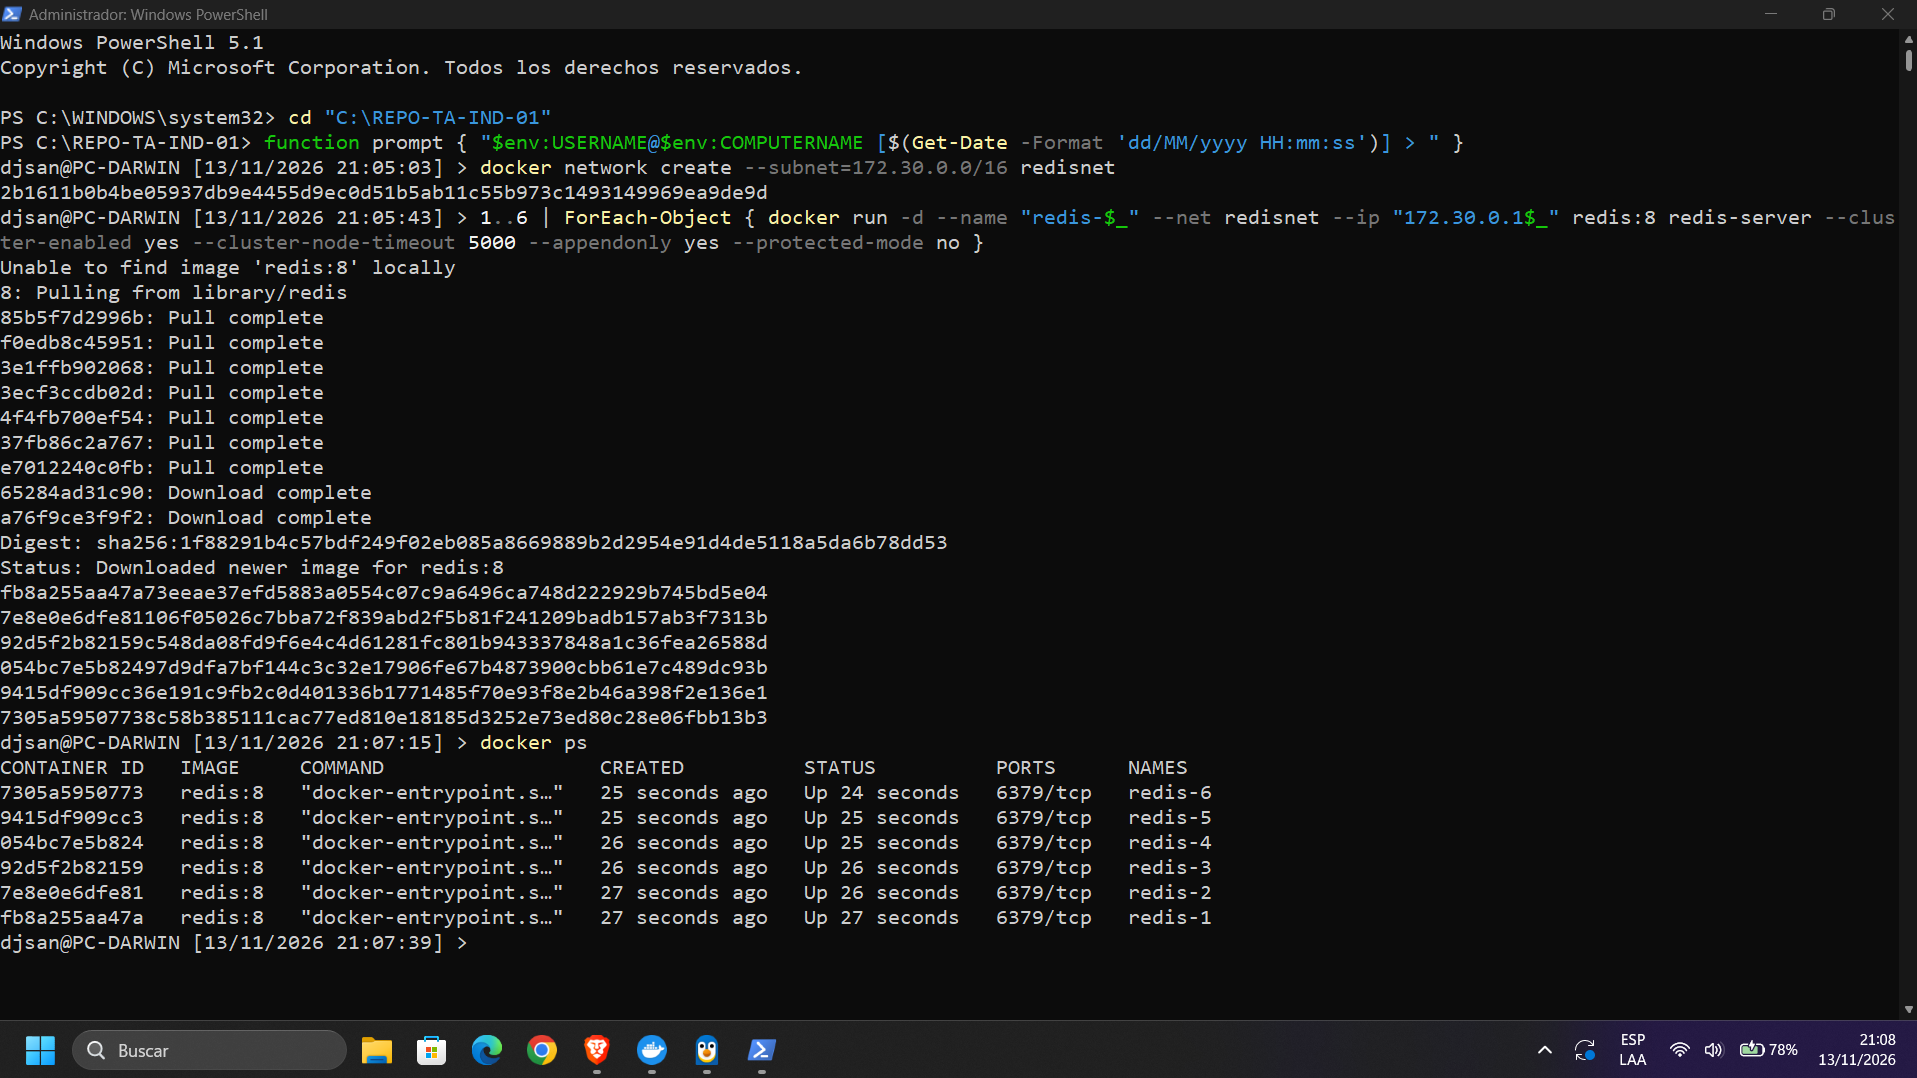
\includegraphics[width=0.9\linewidth]{01-docker-ps.png}
  \caption{Los seis contenedores \texttt{redis-1} a \texttt{redis-6} en
  ejecución (\texttt{docker ps}). Captura propia.}
  \label{fig:dockerps}
\end{figure}

\textbf{Creación del clúster.} El clúster se creó con
\texttt{redis-cli --cluster create} y la opción \texttt{--cluster-replicas 1},
que pide una réplica por maestro. La herramienta repartió los 16\,384 slots en
tres rangos y asignó las réplicas de la Tabla~\ref{tab:nodos}, terminando con
el mensaje \texttt{[OK] All 16384 slots covered} (Figura~\ref{fig:create}).

\begin{figure}[H]
  \centering
  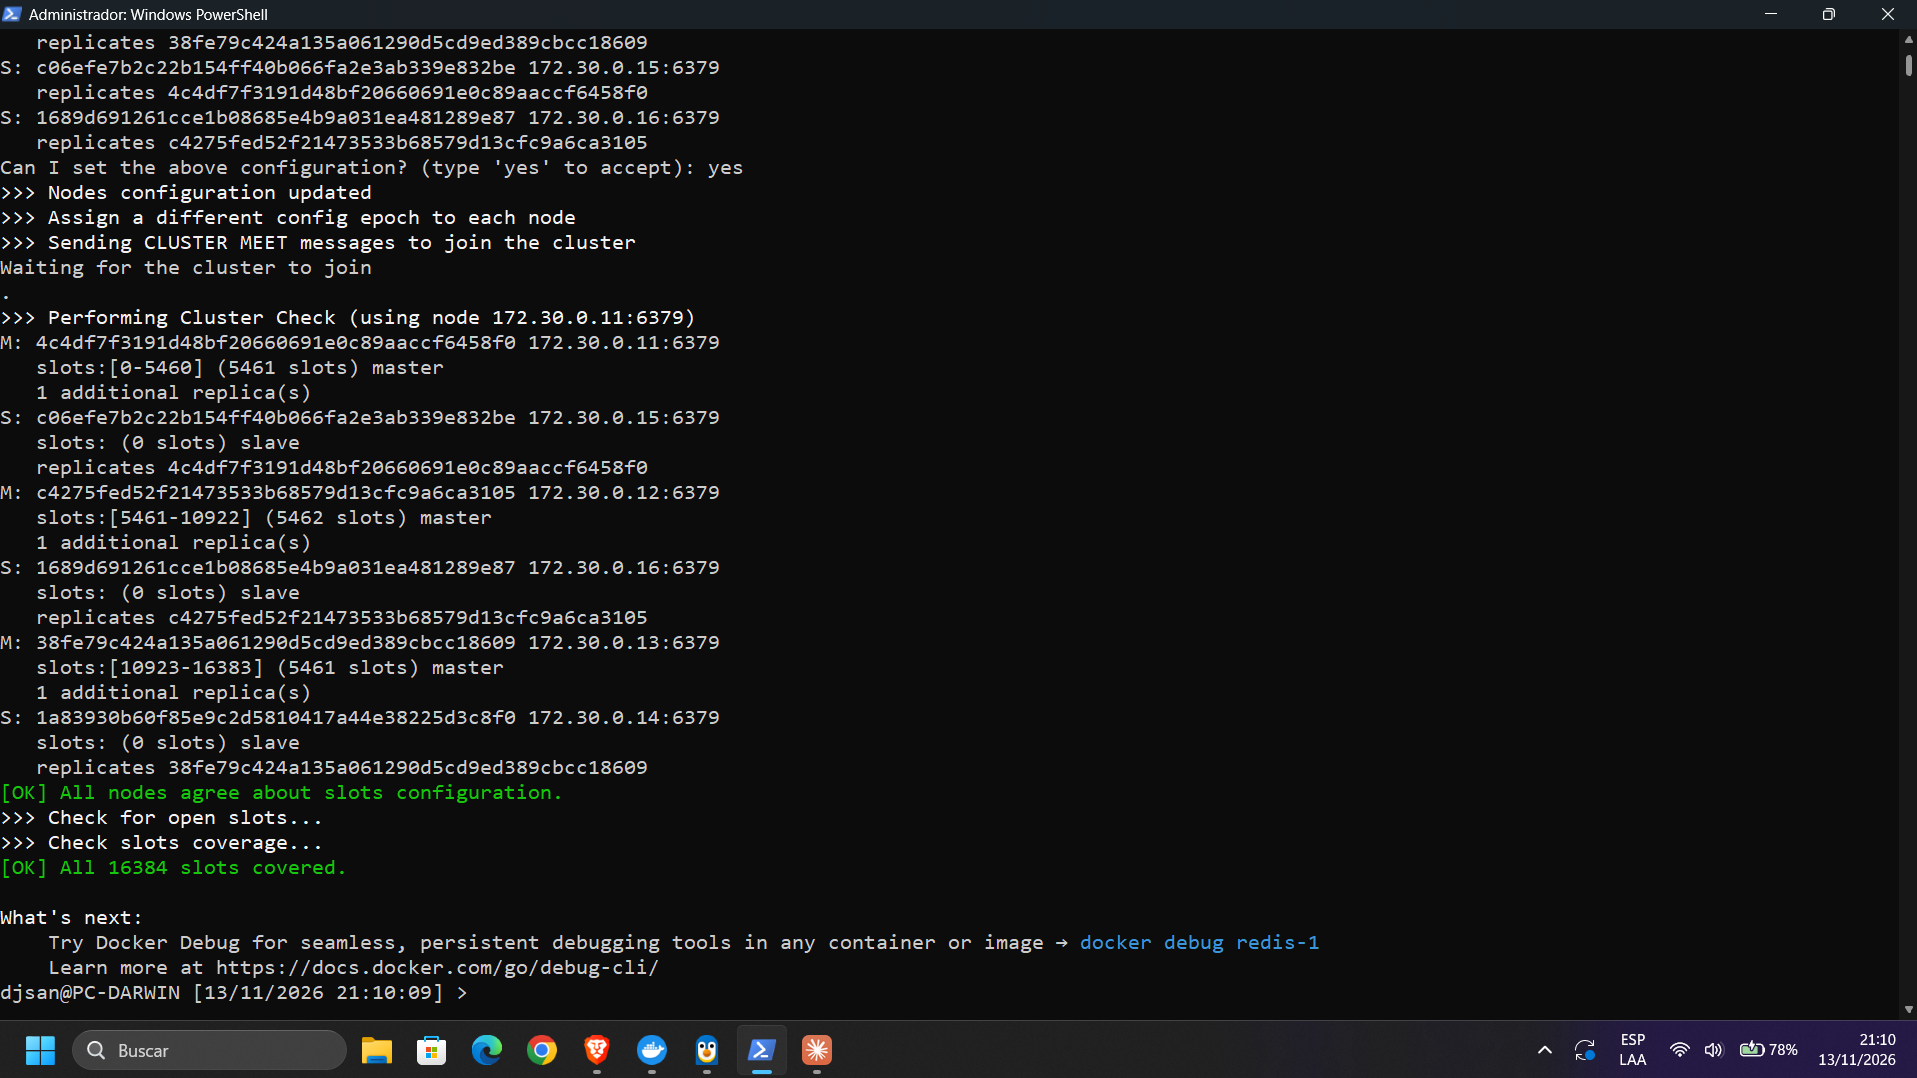
\includegraphics[width=0.9\linewidth]{02-cluster-create.png}
  \caption{Creación del clúster con tres maestros y tres réplicas. Captura
  propia.}
  \label{fig:create}
\end{figure}

\textbf{Estado del clúster.} \texttt{CLUSTER INFO} confirmó
\texttt{cluster\_state:ok}, los 16\,384 slots asignados, seis nodos conocidos
y tres maestros (\texttt{cluster\_size:3}). Los contadores de mensajes
\emph{ping} y \emph{pong} enviados y recibidos (más de 1\,800 de cada tipo en
pocos minutos) son la evidencia del \emph{gossip} por el bus del clúster. En
\texttt{CLUSTER NODES} cada nodo aparece como \texttt{IP:6379@16379}: el
primer puerto atiende a los clientes y el segundo es el bus del clúster
(Figura~\ref{fig:nodes}).

\begin{figure}[H]
  \centering
  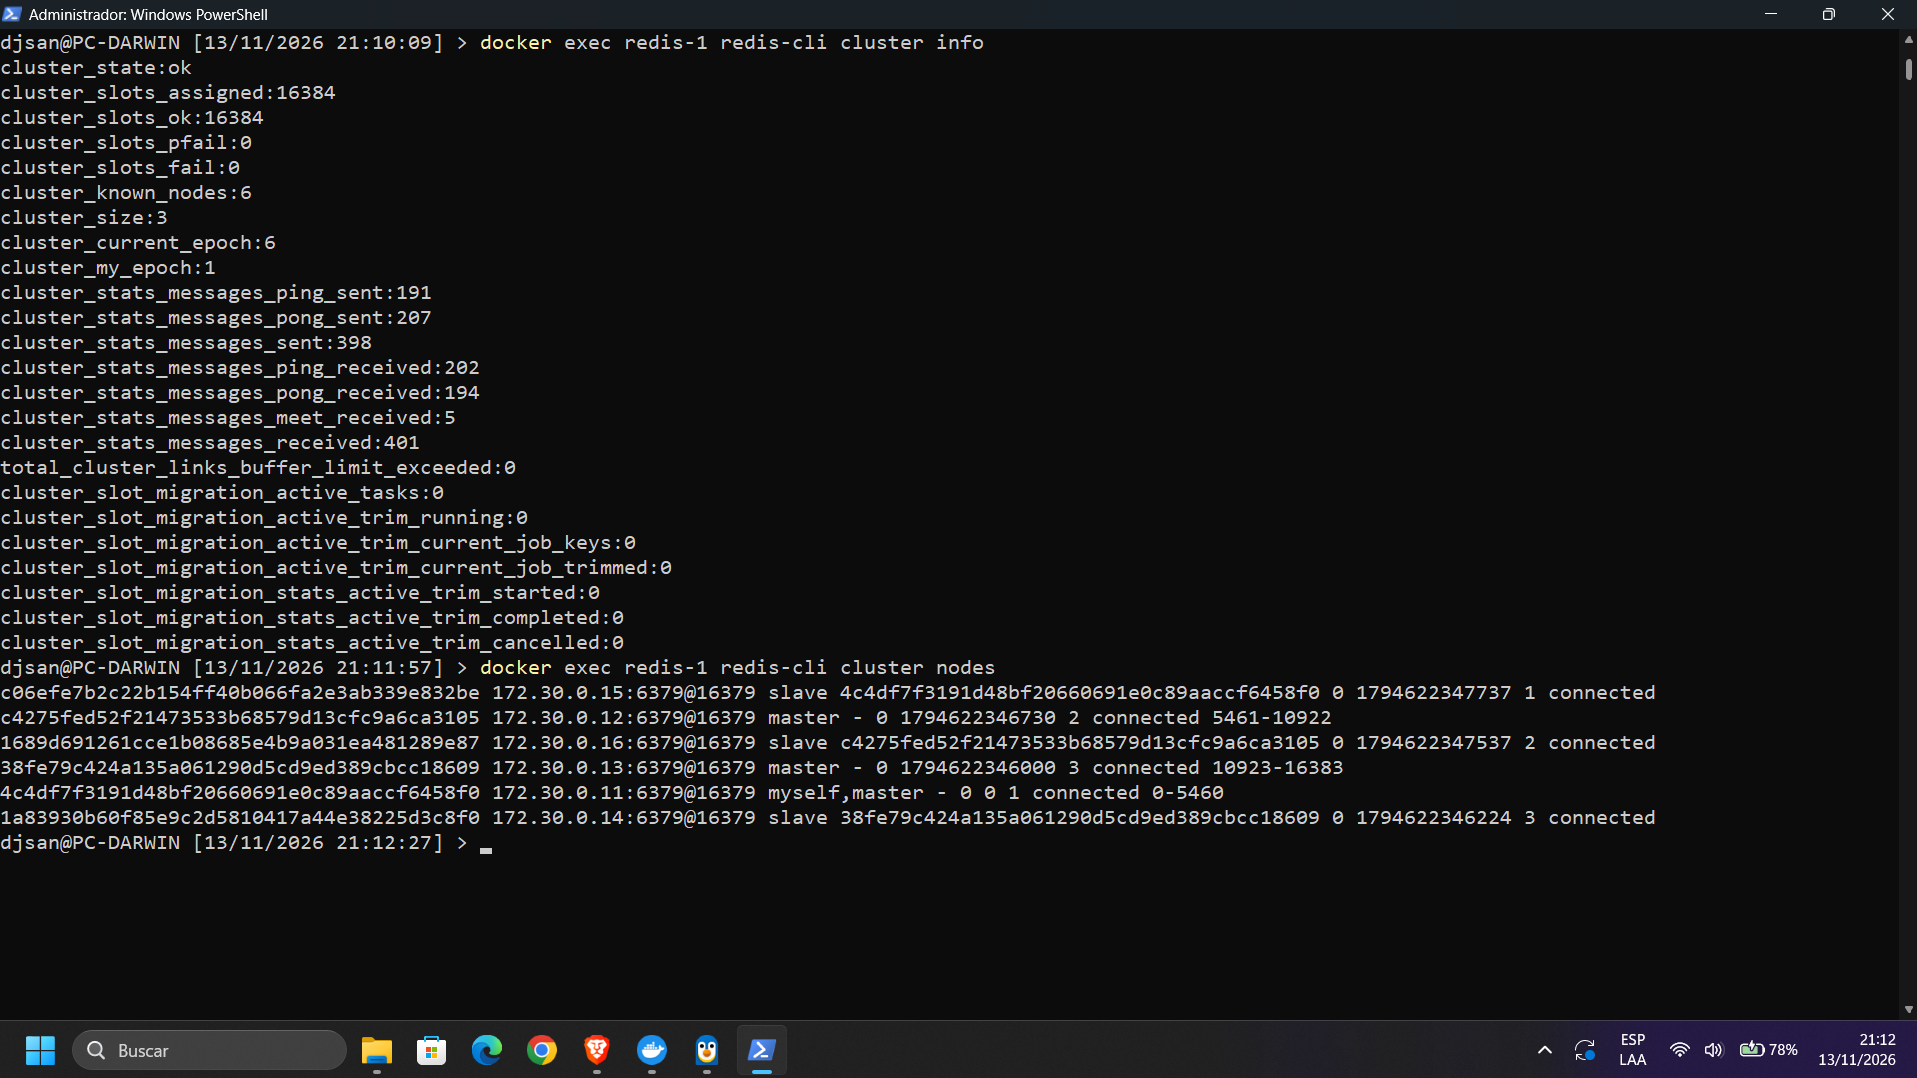
\includegraphics[width=0.9\linewidth]{03-cluster-info-nodes.png}
  \caption{Salida de \texttt{CLUSTER INFO} y \texttt{CLUSTER NODES}.
  Captura propia.}
  \label{fig:nodes}
\end{figure}

\textbf{Escritura y lectura con redirección.} Desde \texttt{redis-1}
(172.30.0.11), con \texttt{redis-cli -c}, se escribieron y leyeron dos
claves. Ninguna pertenecía a ese nodo, así que en ambos casos el clúster
devolvió una redirección y el cliente repitió la petición en el nodo dueño del
slot (Tabla~\ref{tab:claves} y Figura~\ref{fig:redireccion}).

\begin{table}[H]
  \centering
  \caption{Claves de prueba y nodo que las almacena.}
  \label{tab:claves}
  \begin{tabular}{lcl}
    \toprule
    \textbf{Clave} & \textbf{Slot} & \textbf{Nodo dueño} \\
    \midrule
    \texttt{usuario:25}           & 7554  & 172.30.0.12 (maestro B) \\
    \texttt{materia:aplicaciones} & 13574 & 172.30.0.13 (maestro C) \\
    \bottomrule
  \end{tabular}
\end{table}

\begin{figure}[H]
  \centering
  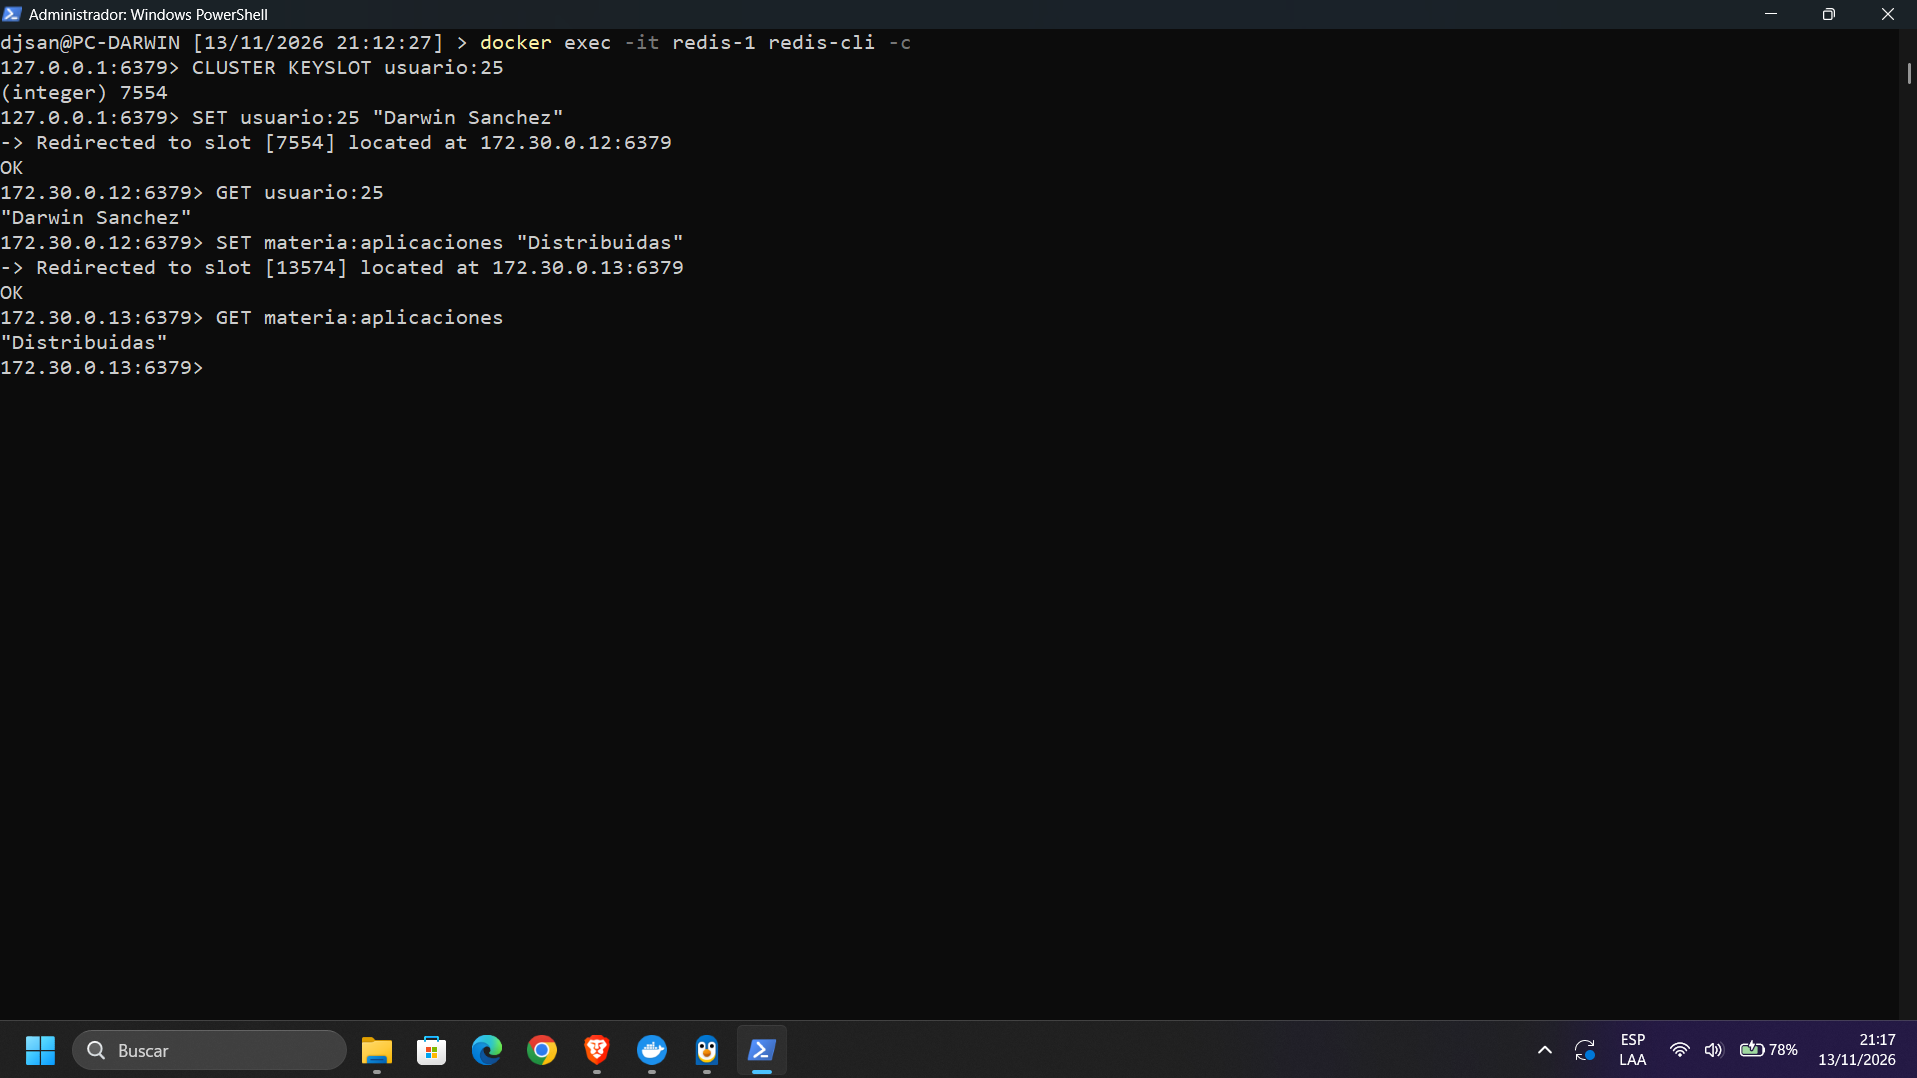
\includegraphics[width=0.9\linewidth]{04-set-get-redireccion.png}
  \caption{Escritura y lectura con redirección entre nodos
  (\texttt{redis-cli -c}). Captura propia.}
  \label{fig:redireccion}
\end{figure}

Esta prueba muestra la transparencia de ubicación \emph{parcial} descrita en
la Tabla~\ref{tab:transparencias}: con la opción \texttt{-c} el usuario
obtiene su dato sin saber dónde está, pero la redirección sigue siendo
visible en la salida, y sin esa opción el cliente recibiría un error
\texttt{MOVED}.

\subsection{Experimento E1: caída de un nodo maestro}

\textbf{Objetivo.} Comprobar qué ocurre con el servicio y con los datos cuando
se cae un nodo maestro: cómo se detecta el fallo, cuánto tarda la
recuperación y si se conserva el dato almacenado.

\textbf{Hipótesis.} Según la especificación, si un maestro deja de responder
durante más de \texttt{cluster-node-timeout}, la mayoría de maestros lo marca
como caído y su réplica es promovida \cite{redis2026clusterspec}. Se esperaba
que el failover tardara algo más de 5\,s, que \texttt{redis-6} (172.30.0.16)
pasara a ser maestro de los slots 5461--10922 y que \texttt{usuario:25}
(slot 7554) siguiera disponible.

\textbf{Procedimiento.} Se registró el estado inicial con
\texttt{CLUSTER NODES} y \texttt{GET usuario:25}. A continuación se detuvo el
contenedor \texttt{redis-2} y, cada 0.5\,s, un bucle de PowerShell consultó
el estado del clúster y el rol de \texttt{redis-6} hasta que este apareció
como maestro:

\begin{lstlisting}
docker stop redis-2
$t0 = Get-Date
do {
  Start-Sleep -Milliseconds 500
  $seg = [math]::Round(((Get-Date) - $t0).TotalSeconds, 1)
  $estado = (docker exec redis-1 redis-cli cluster info |
             Select-String "cluster_state").ToString().Trim()
  $nodo16 = (docker exec redis-1 redis-cli cluster nodes |
             Select-String "172.30.0.16").ToString()
  $rol16 = if ($nodo16 -match " master ") { "MASTER" } else { "replica" }
  Write-Host "$seg s | $estado | redis-6: $rol16"
} until ($rol16 -eq "MASTER")
\end{lstlisting}

Después se comprobó el nuevo estado y la clave, se volvió a encender
\texttt{redis-2} y, tras 10\,s, se revisó su rol. Toda la sesión se grabó con
\texttt{Start-Transcript} (\texttt{experimento/salidas/e1-failover.txt}).

\textbf{Resultados.} En el estado inicial (Figura~\ref{fig:e1inicial})
\texttt{redis-2} era maestro de los slots 5461--10922, \texttt{redis-6} era
su réplica y \texttt{GET usuario:25} devolvía \texttt{"Darwin Sanchez"}. La
Tabla~\ref{tab:e1} resume la evolución tras detener el maestro.

\begin{figure}[H]
  \centering
  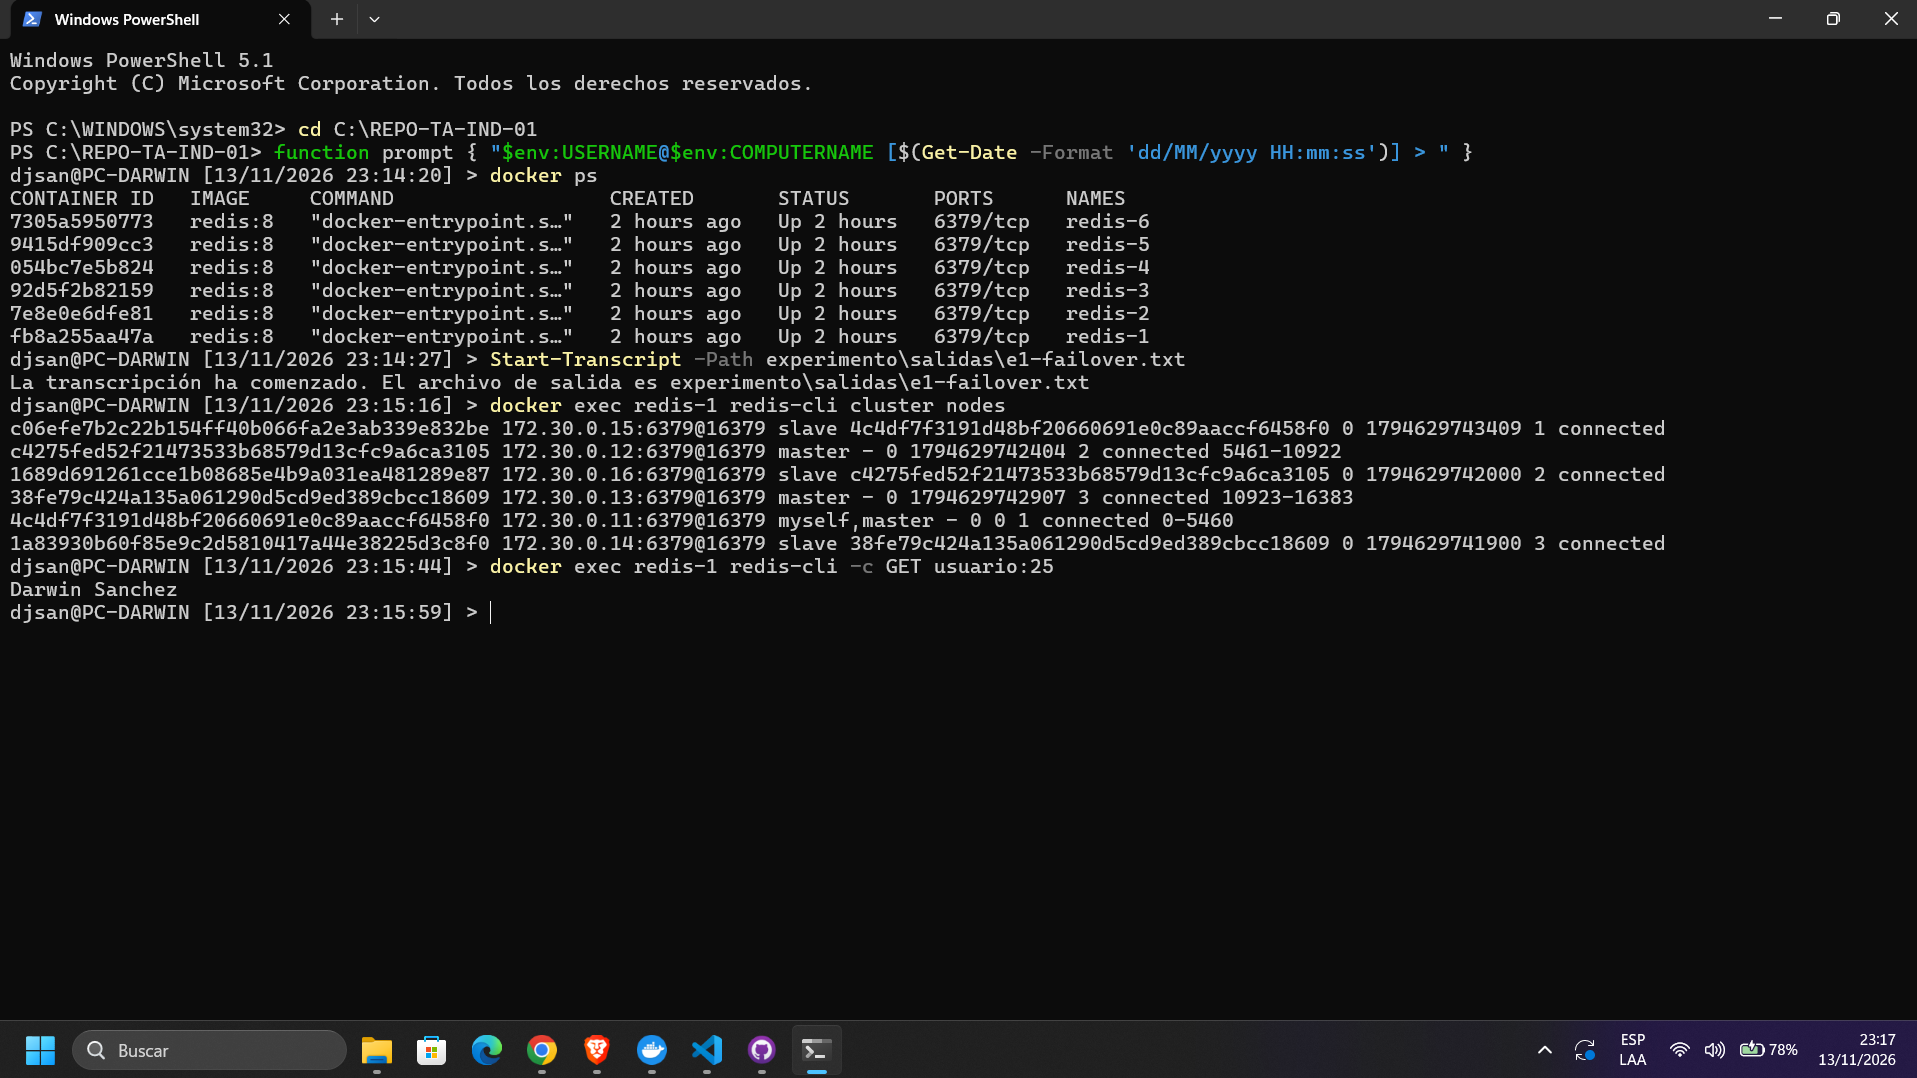
\includegraphics[width=0.9\linewidth]{05-e1-estado-inicial.png}
  \caption{E1: estado inicial del clúster y lectura de \texttt{usuario:25}.
  Captura propia.}
  \label{fig:e1inicial}
\end{figure}

\begin{table}[H]
  \centering
  \caption{Línea de tiempo del failover en el experimento E1.}
  \label{tab:e1}
  \begin{tabular}{lcc}
    \toprule
    \textbf{Tiempo desde \texttt{docker stop}} & \textbf{\texttt{cluster\_state}} & \textbf{Rol de \texttt{redis-6}} \\
    \midrule
    0.6\,s -- 5.5\,s & ok            & réplica \\
    6.2\,s -- 7.1\,s & \textbf{fail} & réplica \\
    7.8\,s           & ok            & \textbf{maestro} \\
    \bottomrule
  \end{tabular}
\end{table}

Tras el failover, \texttt{redis-2} aparecía como \texttt{master,fail},
\texttt{redis-6} era el nuevo maestro de los slots 5461--10922, su época de
configuración pasó de 2 a 7 y \texttt{GET usuario:25} siguió devolviendo el
dato (Figura~\ref{fig:e1failover}). Al reiniciar \texttt{redis-2}, este
volvió al clúster como \emph{réplica} de \texttt{redis-6} y no recuperó su
papel de maestro (Figura~\ref{fig:e1recuperacion}).

\begin{figure}[H]
  \centering
  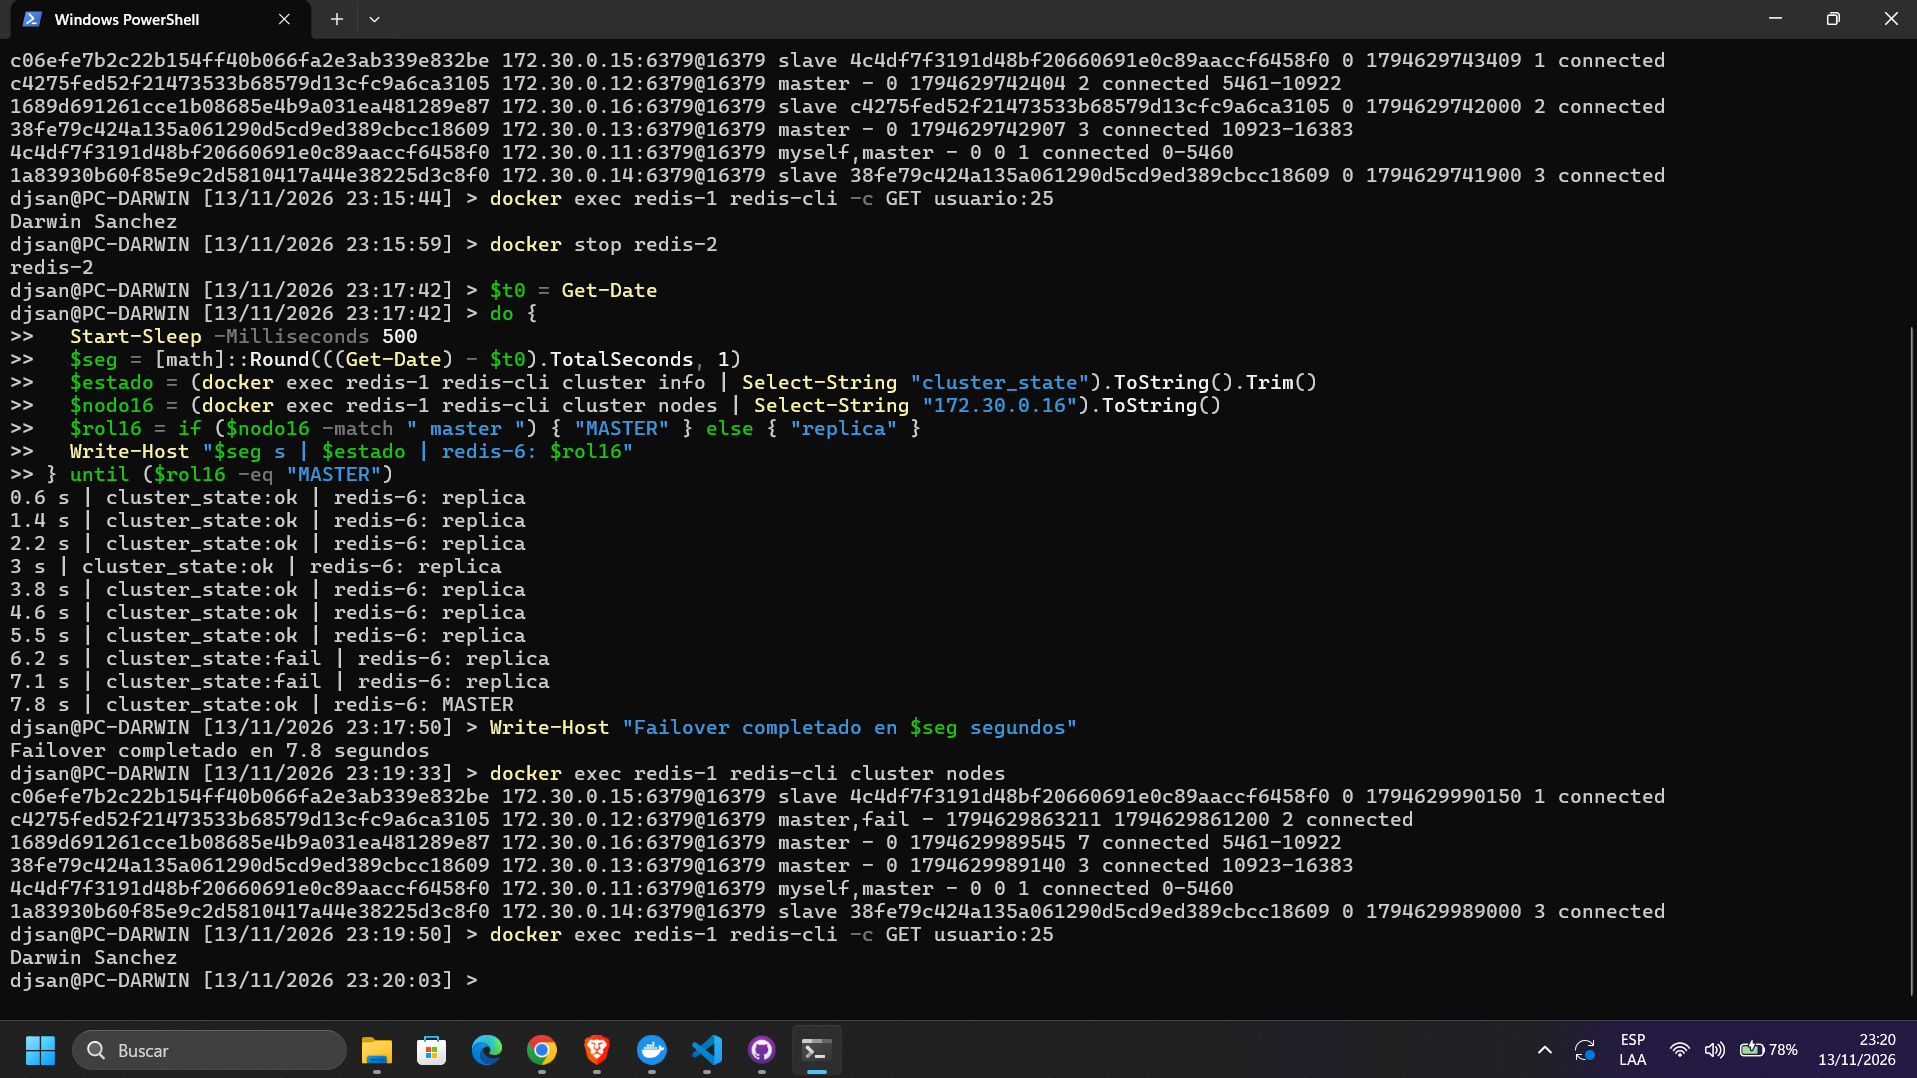
\includegraphics[width=0.9\linewidth]{06-e1-failover.png}
  \caption{E1: línea de tiempo del failover y estado posterior. Captura
  propia.}
  \label{fig:e1failover}
\end{figure}

\begin{figure}[H]
  \centering
  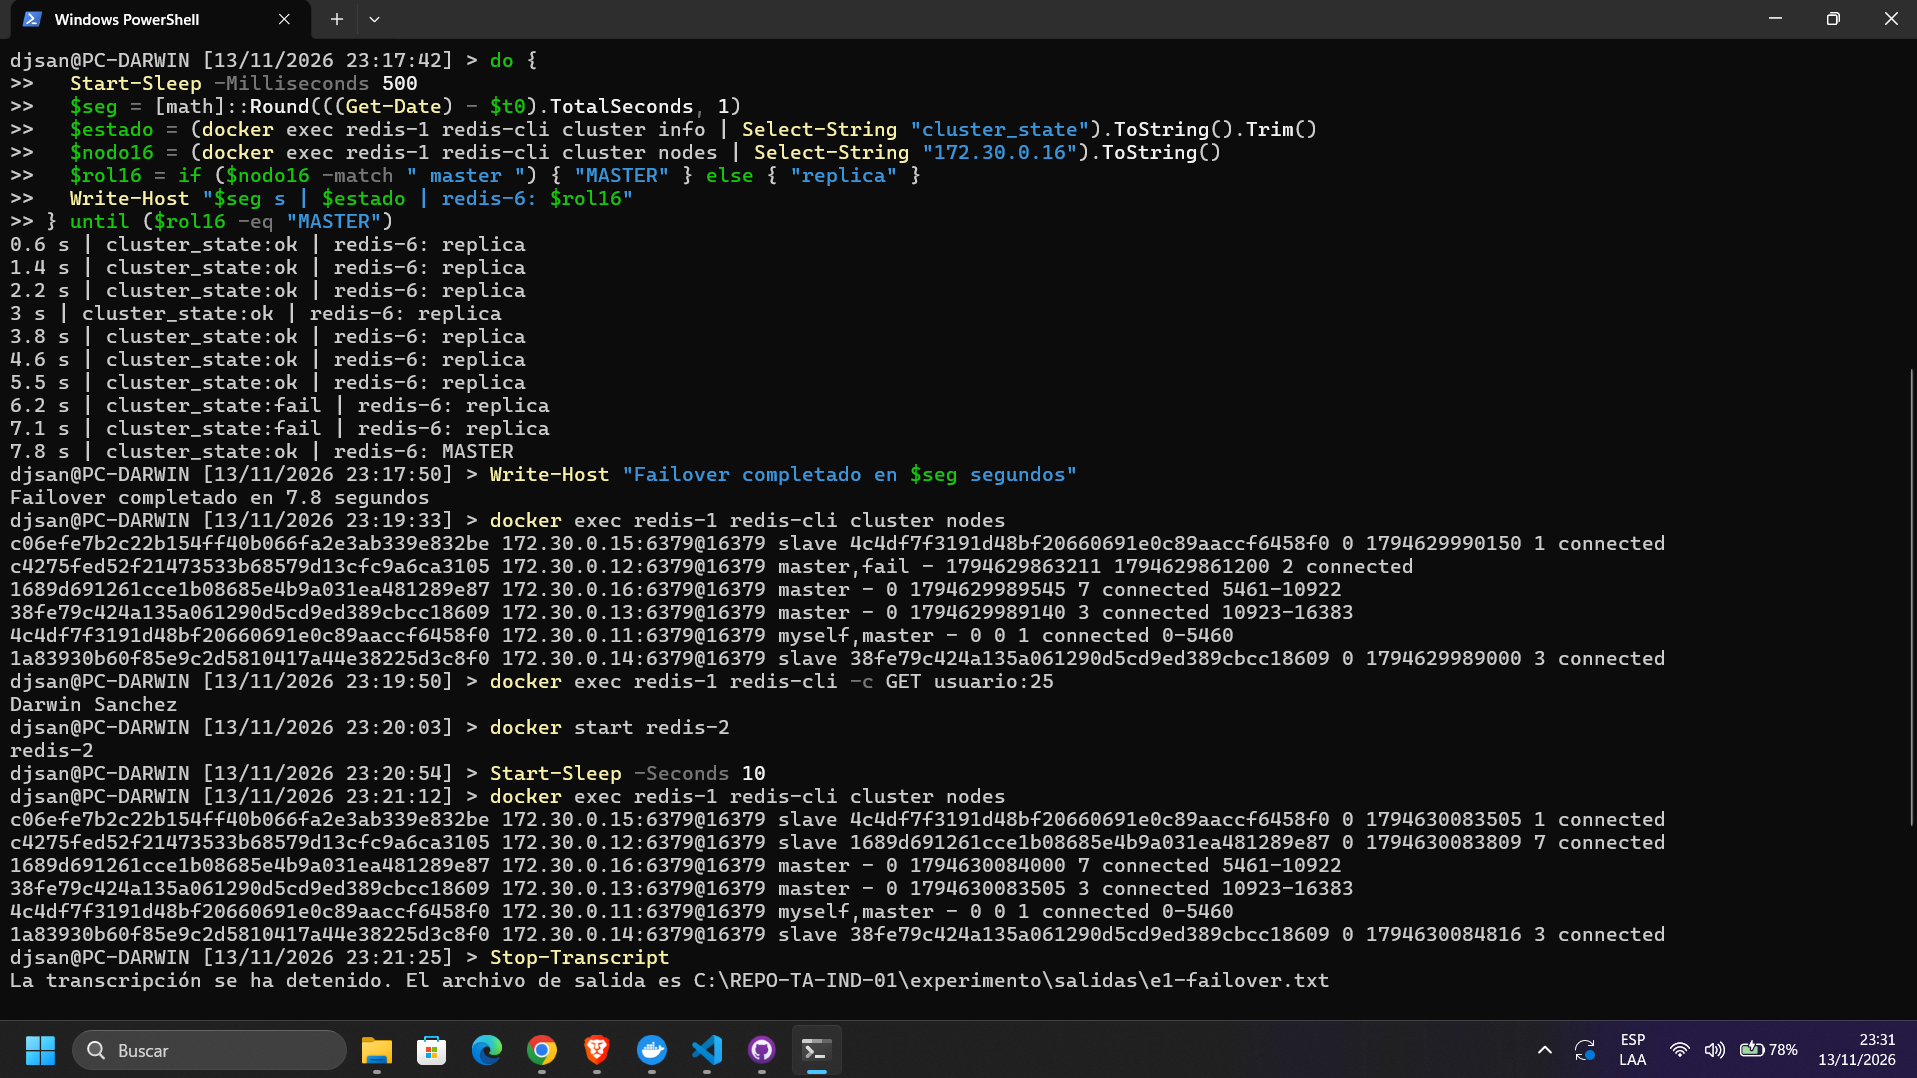
\includegraphics[width=0.9\linewidth]{07-e1-recuperacion.png}
  \caption{E1: \texttt{redis-2} se reincorpora como réplica del nuevo
  maestro. Captura propia.}
  \label{fig:e1recuperacion}
\end{figure}

\textbf{Interpretación.} Los resultados confirman la hipótesis y permiten
observar varios conceptos de la Unidad~1:

\begin{itemize}
  \item \textbf{Detección por \emph{timeout} y mayoría.} El clúster siguió
  en estado \texttt{ok} hasta los 5.5\,s, aunque el nodo ya estaba apagado,
  porque Redis espera el \texttt{cluster-node-timeout} antes de sospechar de
  un nodo y necesita que la mayoría de maestros confirme el fallo. El total de
  7.8\,s corresponde al \emph{timeout} más la confirmación y la votación.
  \item \textbf{Ventana de indisponibilidad.} Durante esos primeros segundos
  el clúster seguía considerando a \texttt{redis-2} dueño de sus slots, de modo
  que una petición sobre \texttt{usuario:25} se habría dirigido a un nodo
  apagado. Esta afirmación se deduce de la especificación, ya que no se midió
  con un cliente durante la ventana.
  \item \textbf{Estado \texttt{fail} y CAP.} Entre 6.2 y 7.1\,s todo el
  clúster dejó de atender consultas porque un rango de slots se quedó sin
  maestro (\texttt{cluster-require-full-coverage yes}). Se sacrificó
  disponibilidad durante un instante, pero sin ganar consistencia fuerte: la
  réplica promovida se actualiza de forma asíncrona.
  \item \textbf{Conservación del dato.} \texttt{usuario:25} se escribió unas
  dos horas antes de la caída y la réplica ya tenía la copia. Si se hubiera
  escrito justo antes, el maestro podría haber confirmado la escritura sin
  enviarla a la réplica, y el dato se habría perdido: es la decisión EL de
  PACELC observada en la práctica.
  \item \textbf{Época de configuración.} El salto de la época de 2 a 7 y el
  regreso de \texttt{redis-2} como réplica muestran cómo Redis evita tener dos
  maestros para los mismos slots: prevalece la configuración más reciente.
\end{itemize}

\textbf{Limitaciones.} Se hizo una sola ejecución, por lo que el tiempo de
failover puede variar entre repeticiones. No se midieron las peticiones de un
cliente durante la ventana de fallo. Además, todos los nodos se ejecutaron en
el mismo equipo, sin la latencia ni las pérdidas de una red real, y no se
probó una partición de red, sino solo la caída de un nodo.

\subsection{Ejemplos en mi propio entorno}

PENDIENTE

% =====================================================================
\section{Comparación con Hazelcast}
\label{sec:comparacion}
% =====================================================================

PENDIENTE

% =====================================================================
\section{Postura crítica}
\label{sec:postura}
% =====================================================================

\textbf{Redis Cluster no es un sistema CP, aunque algunas fuentes lo
clasifiquen así.} La revisión de Ahmed et~al. incluye a Redis entre los
sistemas CP, es decir, entre los que sacrifican disponibilidad para preservar
la consistencia durante una partición \cite[p.~172]{ahmed2023consistency}.
Considero que esta clasificación no se sostiene para Redis Cluster por tres
razones. Primero, la propia especificación reconoce que el clúster no ofrece
consistencia fuerte y que puede perder escrituras ya confirmadas al cliente
\cite{redis2026clusterspec}. Segundo, el estudio de Ferreira et~al. describe a
Redis como un sistema que prioriza la disponibilidad y que solo ofrece un
control opcional de las escrituras con \texttt{WAIT}
\cite[p.~4]{ferreira2024impacts}. Tercero, en mi experimento E1 el clúster sí
dejó de responder durante unos segundos, pero no lo hizo para proteger la
consistencia, sino porque un rango de slots se quedó sin maestro; la réplica
promovida podía no tener las últimas escrituras. Una posible explicación de
la diferencia es que la revisión clasifica a ``Redis'' de forma general, sin
distinguir entre un servidor único, la replicación con Sentinel y Redis
Cluster, ni su configuración. Esto me lleva a una conclusión más general: las
etiquetas CAP de una revisión bibliográfica no deben aceptarse sin comprobar
cómo replica realmente el sistema y con qué configuración se despliega.

\textbf{La decisión PA/EL es acertada para el uso principal de Redis, pero
peligrosa fuera de él.} Para una caché o para sesiones de usuario, perder las
últimas escrituras tras un fallo es tolerable: el dato se vuelve a calcular o
el usuario inicia sesión otra vez, y a cambio se obtienen respuestas en
fracciones de milisegundo. En cambio, usar Redis Cluster como almacén
principal de datos que no se pueden perder, como un saldo o un inventario, sería
un error de diseño. El comando \texttt{WAIT} no resuelve el problema, porque
no garantiza consistencia fuerte \cite{redis2026clusterspec} y, según las
mediciones de Ferreira et~al., reduce el rendimiento de forma drástica cuando
los nodos están en distintas regiones \cite{ferreira2024impacts,
ferreira2025benchmarking}. En ese caso se pierde la principal ventaja de Redis
sin obtener las garantías de un sistema realmente consistente.

\textbf{La transparencia de fallos es menor de lo que parece.} Desde el
cliente, el failover del experimento E1 fue casi invisible: la clave siguió
disponible y no hubo que cambiar nada. Pero la ventana de 7.8\,s se obtuvo con
un \texttt{cluster-node-timeout} de solo 5\,s y con todos los nodos en el
mismo equipo; con el valor por defecto de la configuración de Redis
(15\,s) y una red real, la indisponibilidad parcial sería mayor. Reducir el
\emph{timeout} acelera la recuperación, pero aumenta el riesgo de declarar
caído a un nodo que solo estaba lento. No hay un valor correcto universal: es
otro compromiso que el administrador debe ajustar según su red.

\textbf{La tolerancia a fallos no termina en el servidor.} El incidente de
ChatGPT de 2023 ocurrió con los servidores Redis funcionando correctamente: el
fallo estaba en la biblioteca cliente, que devolvió a un usuario la respuesta
destinada a otro \cite{openai2023outage}. Los mecanismos de Redis Cluster
están diseñados para detectar nodos que dejan de responder, no respuestas
incorrectas. Por eso, al evaluar un sistema distribuido es necesario
considerar todo el ecosistema (clientes, bibliotecas y configuración), y no
solo las garantías que promete el servidor.

\textbf{Valoración general.} Redis Cluster es un diseño coherente: renuncia a
un coordinador central y a la consistencia fuerte para ofrecer baja latencia,
escalabilidad horizontal y una recuperación automática y rápida ante la caída
de un nodo. Su principal debilidad es que estos compromisos no siempre son
evidentes para quien lo usa: el cliente debe entender los slots y las
redirecciones, y quien diseña el sistema debe saber que una escritura
confirmada puede perderse. Bien entendido, es una herramienta adecuada para
datos rápidos y reconstruibles; mal entendido, puede provocar pérdidas de
datos que el sistema nunca prometió evitar.

% =====================================================================
\section{Conclusiones}
\label{sec:conclusiones}
% =====================================================================

PENDIENTE

% =====================================================================
\section*{Declaración de uso de inteligencia artificial}
\addcontentsline{toc}{section}{Declaración de uso de inteligencia artificial}
% =====================================================================

Durante la elaboración de este trabajo se utilizó el asistente de
inteligencia artificial Claude (Anthropic) como herramienta de apoyo, en las
siguientes tareas:

\begin{itemize}
  \item \textbf{Selección de los sistemas:} propuesta de sistemas candidatos
  que no estuvieran en la lista de exclusiones. La elección final de Redis
  Cluster y Hazelcast fue mía.
  \item \textbf{Bibliografía:} búsqueda de artículos de acceso abierto,
  verificación de sus datos (autores, revista, volumen, páginas y DOI) y
  elaboración del archivo \texttt{referencias.bib}. Abrí cada DOI para
  comprobar que las referencias existen y son correctas. También me orientó
  sobre qué páginas de los artículos leer; la lectura, la selección y el
  subrayado de las capturas del Anexo~B los hice yo.
  \item \textbf{Comprensión de conceptos:} explicación de los \emph{hash
  slots}, las réplicas y el failover, apoyada en un diagrama interactivo de
  prueba.
  \item \textbf{Entorno y experimentos:} guía para instalar Docker Desktop y
  WSL~2, resolver los errores de instalación y preparar los comandos del
  despliegue y del experimento E1. Todos los comandos los ejecuté yo en mi
  equipo; las capturas y las salidas son propias.
  \item \textbf{Diagramas:} generación de un diagrama de referencia visual
  de la arquitectura. El diagrama final de la Figura~\ref{fig:arquitectura}
  lo construí yo en draw.io, y el esquema del Anexo~A lo dibujé a mano.
  \item \textbf{Redacción:} apoyo en la documentación del experimento E1 y su
  interpretación, y en la redacción de la introducción, la arquitectura, el
  análisis de la Unidad~1, la experimentación y la postura crítica de este
  informe.
\end{itemize}

Todo el contenido fue revisado por el autor, quien asume la responsabilidad
total sobre las afirmaciones, los datos y las conclusiones presentados.

% =====================================================================
\printbibliography[heading=bibintoc, title={Referencias}]
% =====================================================================

\appendix
\section{Anexo A: esquema inicial a mano}

\begin{figure}[H]
  \centering
  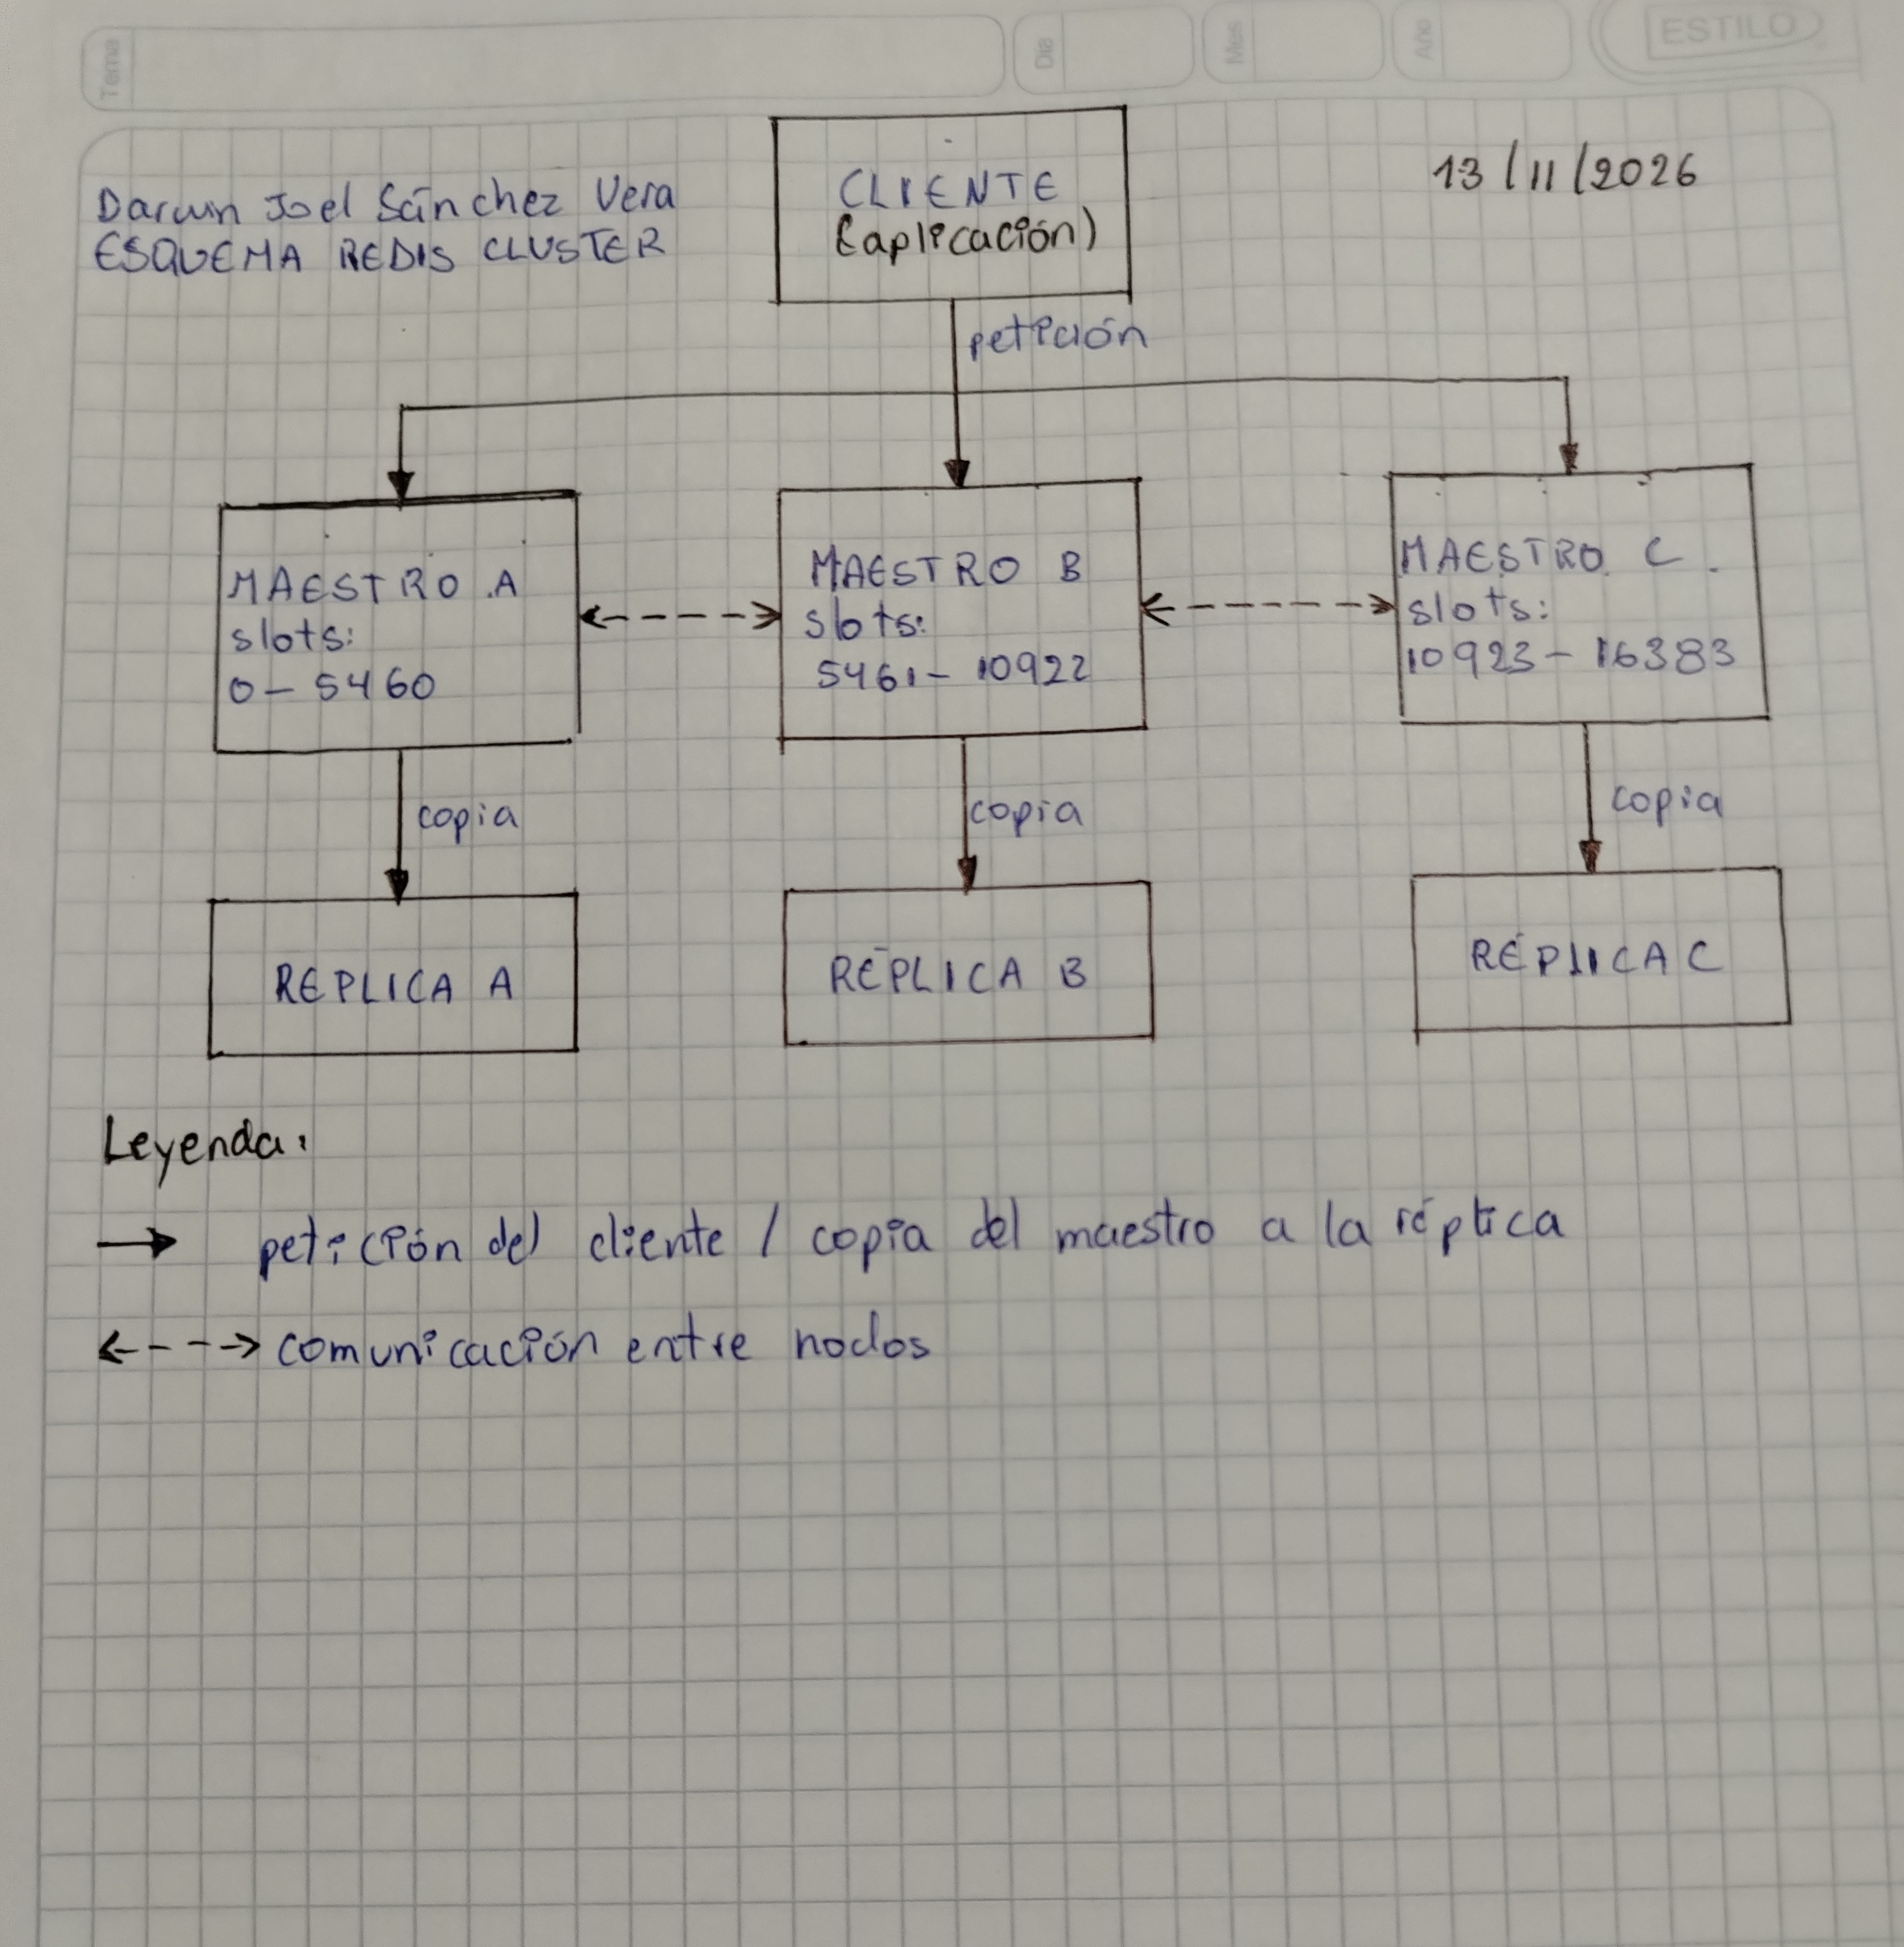
\includegraphics[width=0.85\linewidth]{anexo-a-esquema-a-mano.jpeg}
  \caption{Esquema inicial de la arquitectura de Redis Cluster dibujado a
  mano, con nombre y fecha.}
  \label{fig:anexoA}
\end{figure}

\section{Anexo B: lecturas subrayadas}

\begin{figure}[H]
  \centering
  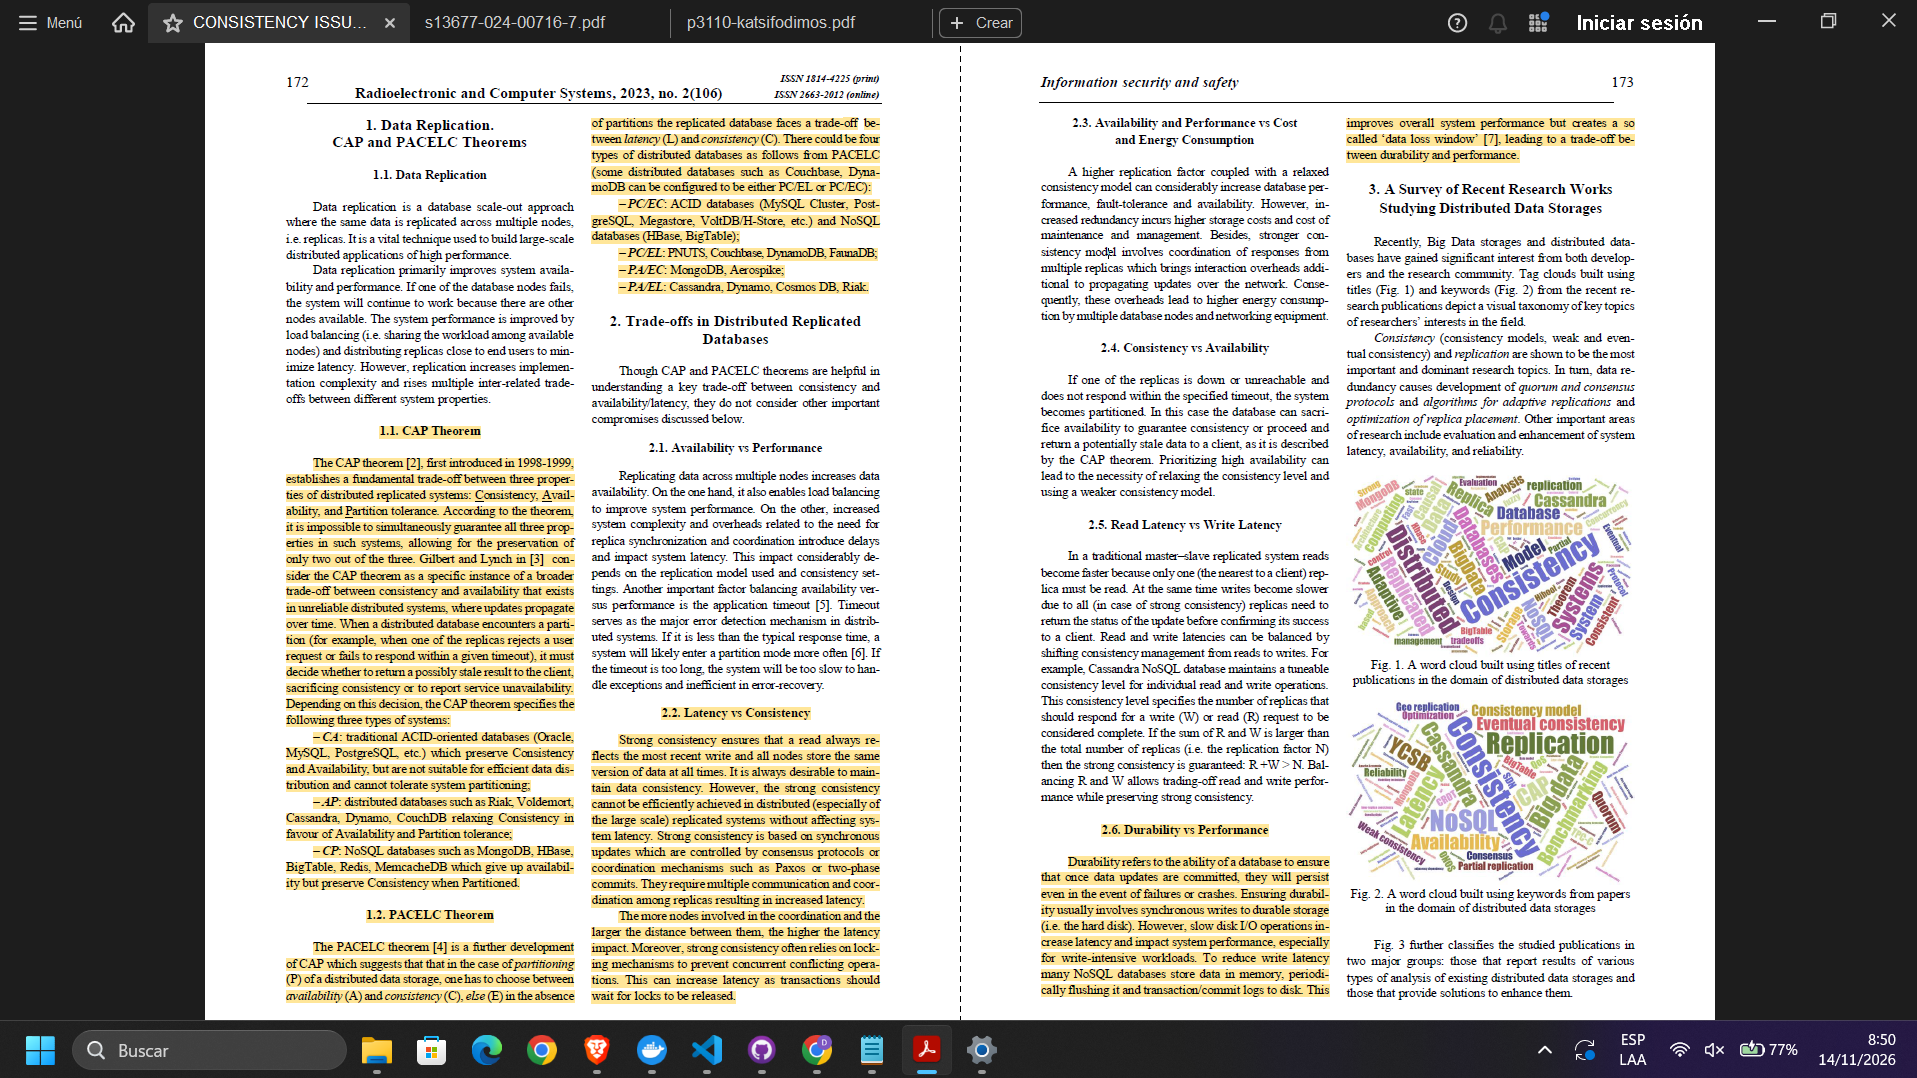
\includegraphics[width=\linewidth]{01-ahmed2023-p172-173-cap-pacelc.png}
  \caption{Ahmed et al. \cite{ahmed2023consistency}, pp.~172--173: teoremas
  CAP y PACELC, clasificación de Redis como CP, latencia frente a consistencia
  y durabilidad.}
\end{figure}

\begin{figure}[H]
  \centering
  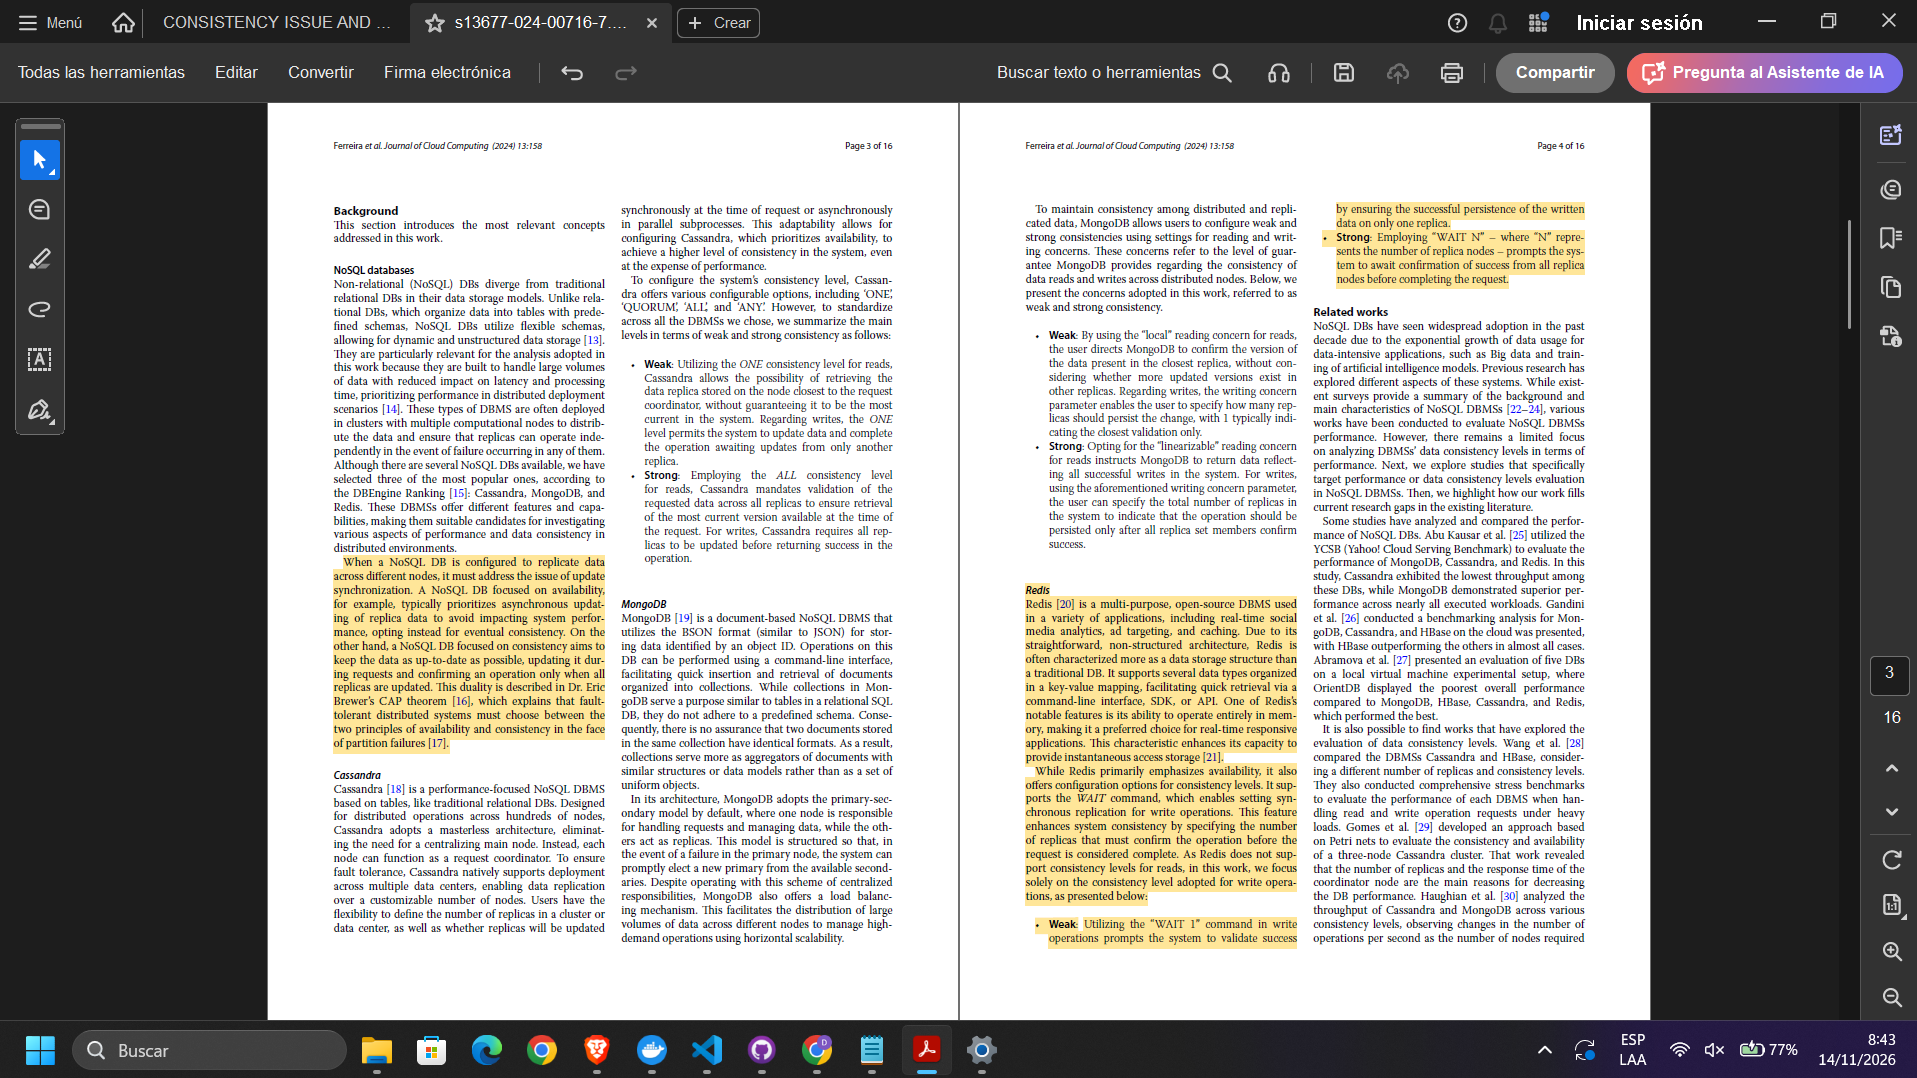
\includegraphics[width=\linewidth]{02-ferreira2024-p3-4-cap-redis-wait.png}
  \caption{Ferreira et al. \cite{ferreira2024impacts}, pp.~3--4: teorema CAP y
  configuración de la consistencia de Redis con \texttt{WAIT}.}
\end{figure}

\begin{figure}[H]
  \centering
  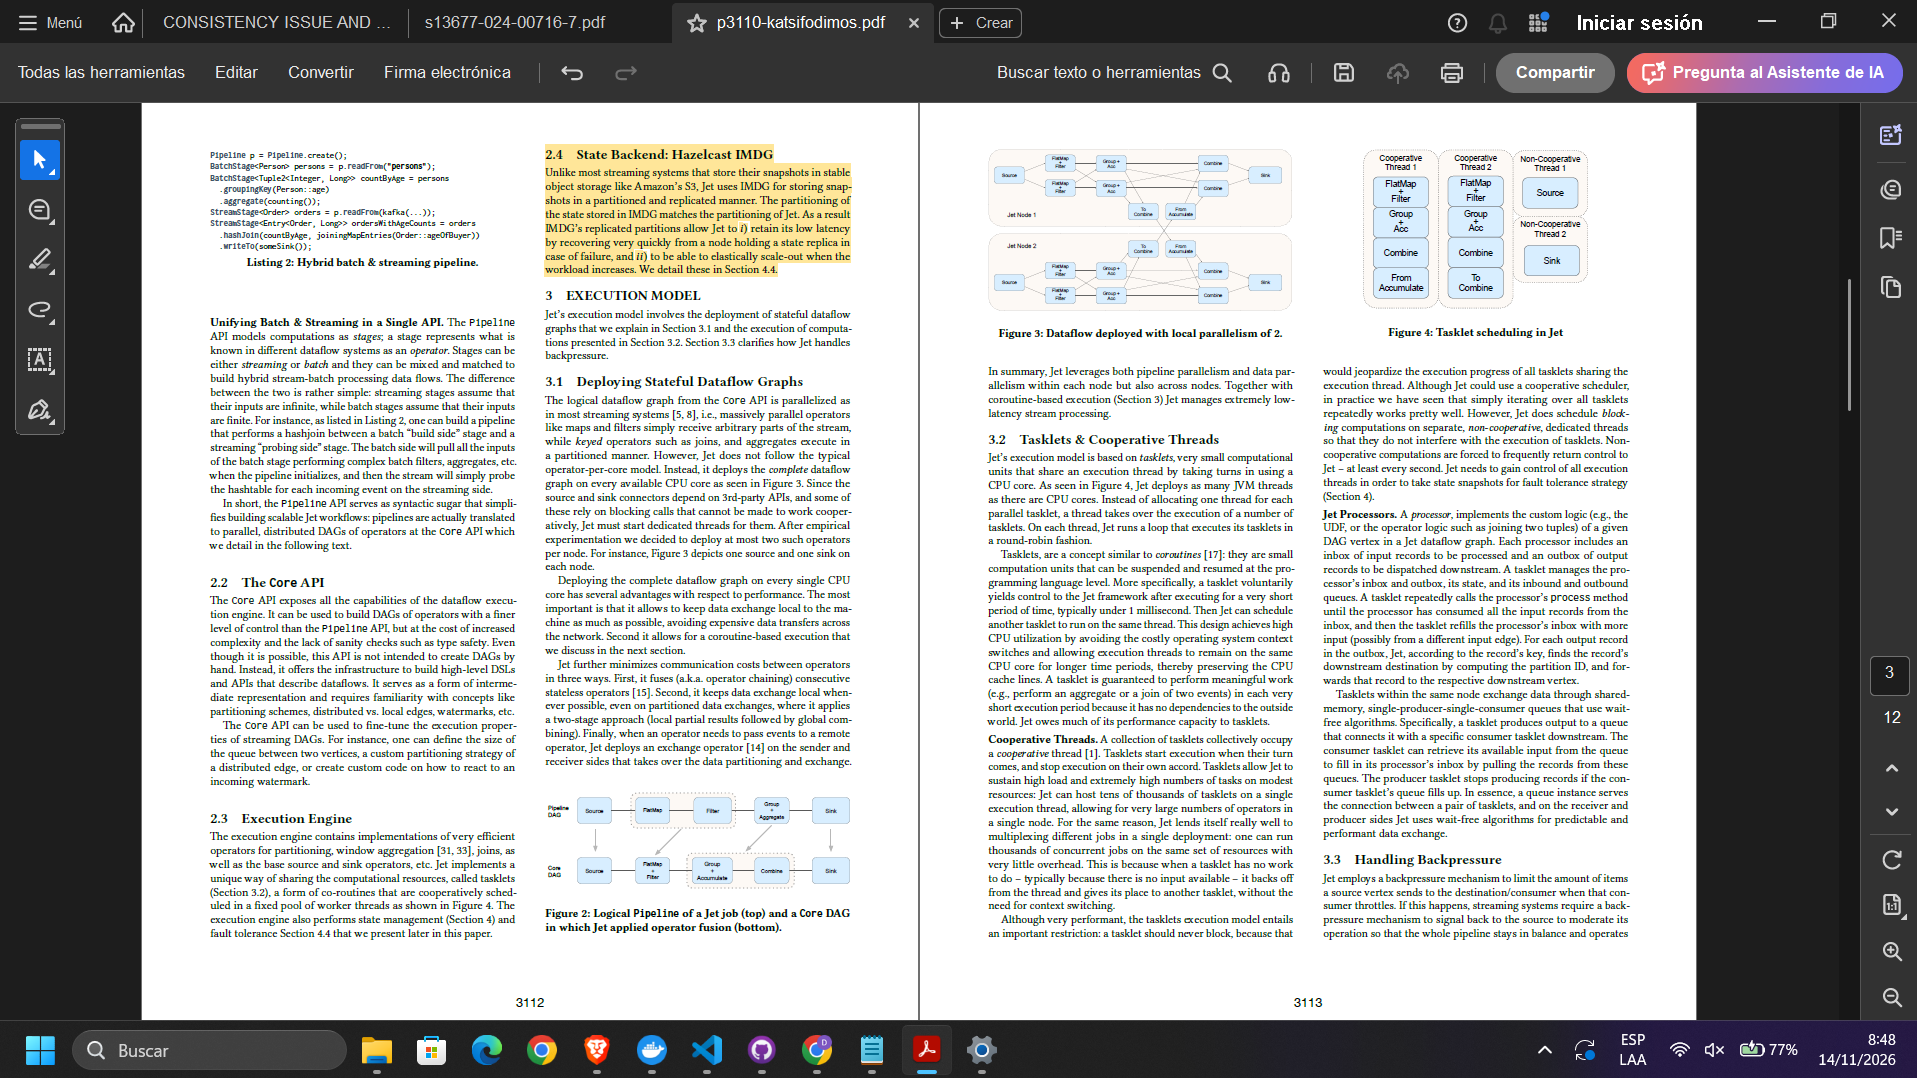
\includegraphics[width=\linewidth]{03-gencer2021-p3112-state-backend.png}
  \caption{Gencer et al. \cite{gencer2021hazelcastjet}, p.~3112: Hazelcast IMDG
  como almacén de estado particionado y replicado.}
\end{figure}

\begin{figure}[H]
  \centering
  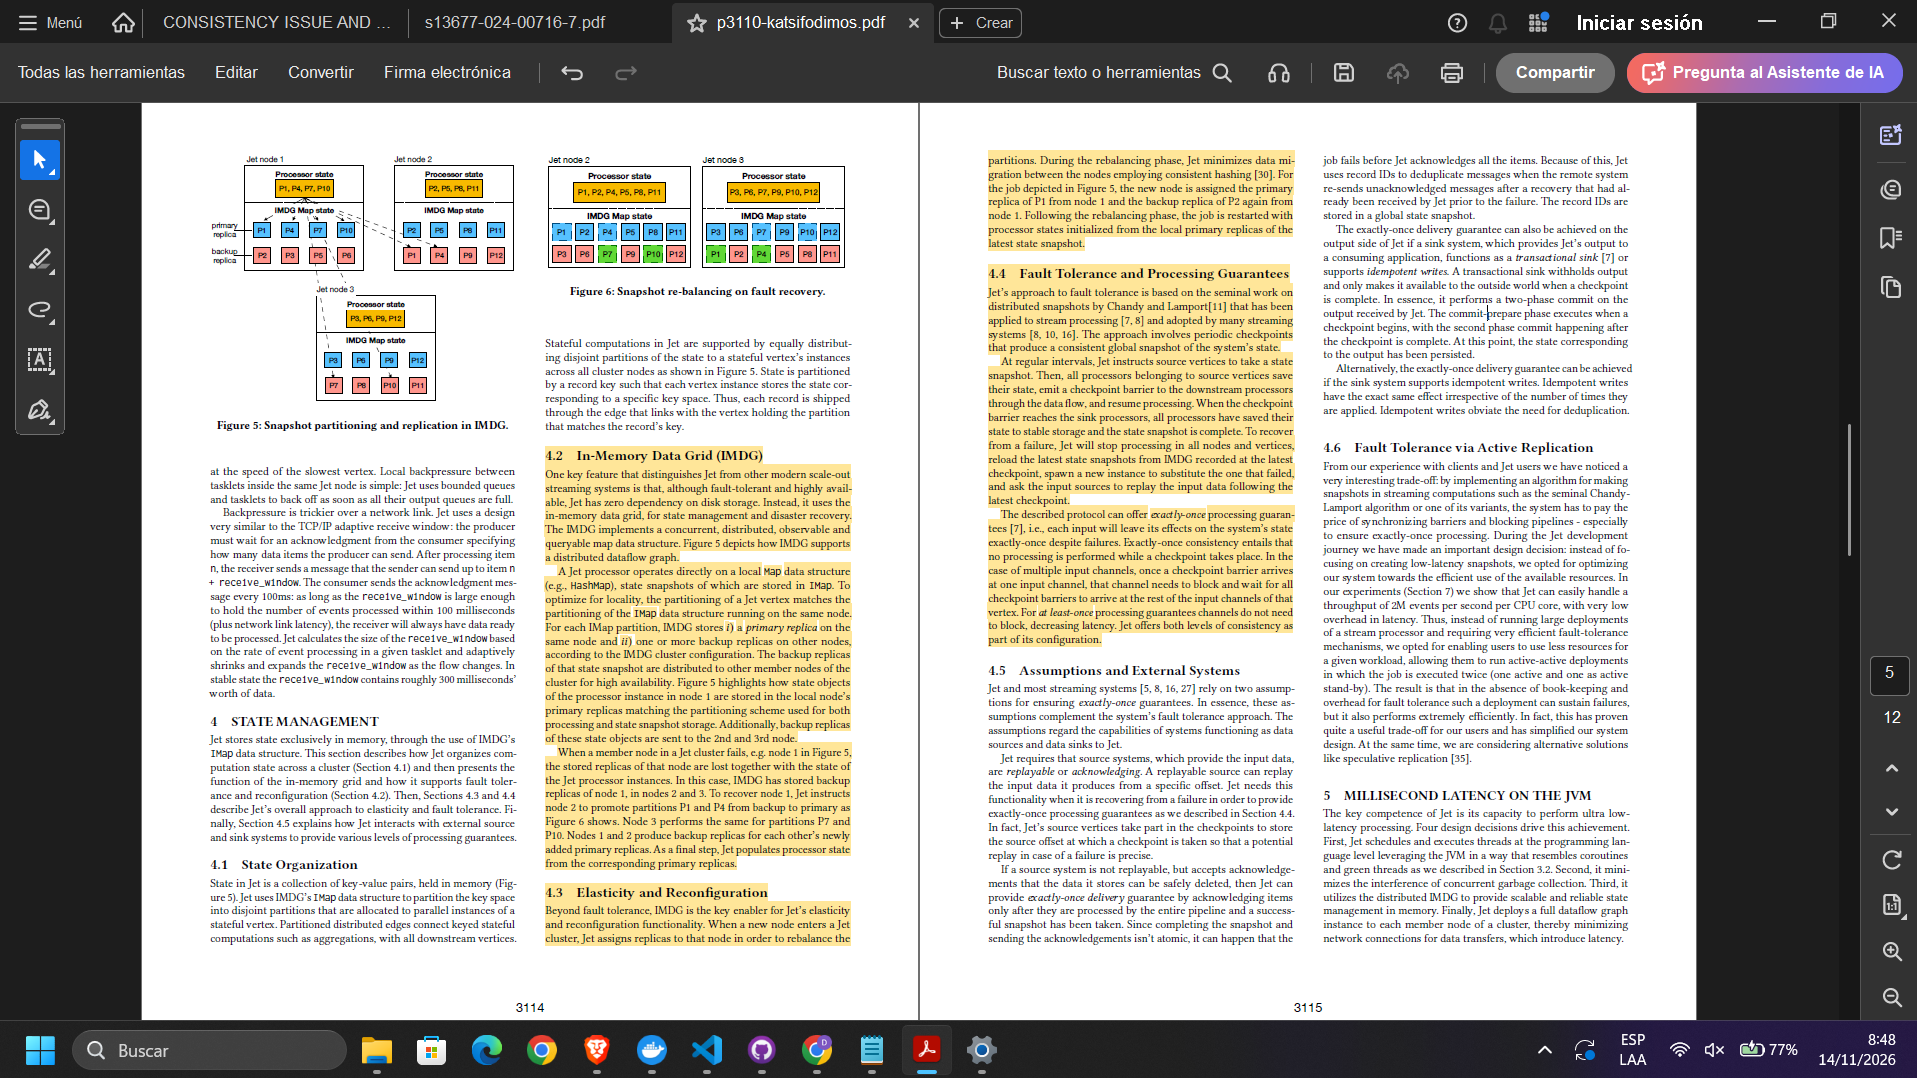
\includegraphics[width=\linewidth]{04-gencer2021-p3114-3115-hazelcast-imdg.png}
  \caption{Gencer et al. \cite{gencer2021hazelcastjet}, pp.~3114--3115: réplicas
  primarias y de respaldo en IMDG, rebalanceo y tolerancia a fallos.}
\end{figure}

\end{document}
